% !TEX TS-program = xelatex
% !BIB program = bibtex
% !TEX encoding = UTF-8 Unicode

\documentclass[
  twoside,
  openright,
  degree    = master,               % degree = master | doctor
  language  = english,              % language = chinese | english
  fontset   = template,             % fontset = default | template | system | overleaf
  watermark = false,                 % watermark = true | false
  doi       = false,                 % doi = true | false
]{ntuthesis}

% !TeX root = ./main.tex

% --------------------------------------------------
% 資訊設定(Information Configs)
% --------------------------------------------------

\ntusetup{
  university*   = {National Taiwan University and Academia Sinica},
  university    = {國立臺灣大學},
  college       = {電機資訊學院暨中央研究院},
  college*      = {College of Electrical Engineering and Computer Science},
  institute     = {資料科學學位學程},
  institute*    = {Data Science Degree Program},
  title         = {自監督學習於圖神經網路:實驗與分析},
  title*        = {Training Graph Neural Networks via Self-Supervised Learning: Experiments and Analysis},
  author        = {何青儒},
  author*       = {Ching-Ru Ho},
  ID            = {R09946006},
  advisor       = {顏佐榕\,博士、沈俊嚴 \,博士},
  advisor*      = {Tso-Jung Yen Ph.D., Chun-Yen Shen Ph.D.},
  date          = {2022-08-01},         % 若註解掉,則預設為當天
  oral-date     = {2022-08-01},         % 若註解掉,則預設為當天
  DOI           = {m},
  keywords      = {自監督學習、圖神經網路、自監督編碼器},
  keywords*     = {self-supervised learning, graph neural network, encoder training},
}

% --------------------------------------------------
% 加載套件(Include Packages)
% --------------------------------------------------
\usepackage{tabularx}
\usepackage[sort&compress]{natbib}      % 參考文獻
\usepackage{amsmath, amsthm, amssymb}   % 數學環境
\usepackage{ulem, CJKulem}              % 下劃線、雙下劃線與波浪紋效果
\usepackage{booktabs}                   % 改善表格設置
\usepackage{multirow}                   % 合併儲存格
\usepackage{diagbox}                    % 插入表格反斜線
\usepackage{array}                      % 調整表格高度
\usepackage{longtable}                  % 支援跨頁長表格
\usepackage{paralist}                   % 列表環境
\usepackage{makecell}

% \usepackage{subfig,epsfig,tikz,float}
% \usepackage{booktabs,multicol,multirow,tabularx,array}     

\usepackage{caption} 
\captionsetup[table]{skip=10pt}

\usepackage{lipsum}                     % 英文亂字
\usepackage{zhlipsum}                   % 中文亂字

% --------------------------------------------------
% 套件設定(Packages Settings)
% --------------------------------------------------


\begin{document}

% 封面與口試審定
% Cover and Verification Letter
\makecover                          % 論文封面(Cover)
\makeverification                   % 口試委員審定書(Verification Letter)

% 致謝與論文摘要
% Acknowledgement and Abstract
% !TeX root = ../main.tex

\begin{acknowledgement}

研究所的日子實在過得飛快,當初排隊領新學生證的回憶彷彿還歷歷在目,卻又在轉瞬間迎接這個即將與學校告別的仲夏。本篇論文得以順利地付梓成冊,一路上真的承蒙很多人的幫忙與鼓勵。在這裡,我想試著用有限的頁數和粗淺的文筆,向這些人表達我無限的感激和敬意。

首先,我要感謝我的指導教授顏佐榕老師。顏老師給予了我在時間規劃上充足的自由,並適時地提供我研究方向的建議與論文寫作的引導,讓我能依照自己的步調,很彈性地嘗試自己想挑戰的事情、摸索自己有興趣的議題。此外,顏老師在日常中的關懷備至、以及每次 meeting 後的閒話家常,也常常讓我覺得自己很幸運能成為您的學生,在此向您致上誠摯的謝意。

感謝我的共同指導教授沈俊嚴老師、口試委員杜憶萍老師、黃冠華老師以及黃信誠老師。撰寫論文是一趟孤獨的長途旅程,時常會有自己沒注意到的盲點或是問題存在,正所謂當局者迷、旁觀者清,若旁人能夠適時的給予提點或建議,將使文章的內容臻於完善,謝謝以上老師們對這篇論文的指教與討論。

再者,也要珍惜這幾年一路陪伴我的好友們,時而分享笑點自娛娛人,時而承擔我壓力的緩衝劑。謝謝吳調亭霖、治翔法師、張檢子儀、前和解律師每週的言論自由日,一起吃壽司、一起踩點、一起擺拍、一起唱K、一起製圖、一起討拍,為煢煢的研究生活帶來不少歡樂,也讓我順利地帶走了兩隻大壽司抱枕,祝福未來大家的人生旅途都能充滿刺激。

謝謝遠在日本的李公亦修三不五時捎來奇葩點子,雖然有時候真的領先人類文明太多年,但每每都能讓我嘆為觀止、增廣見聞;謝謝 Iris 在職涯與藝術方面的啟發與討論,偶爾帶給我迷一般的自信心,或多或少影響了我的眼界和思考模式;謝謝 Hina 在我遇到各種變故的那些日子裡,成為我可靠的傾訴對象,把我從迷航的邊緣救了回來;謝謝芊妤、新愷、湘斌的日常玩笑與取暖,雖然因為疫情的關係有點久沒揪小火鍋了,但與你們的小窗窗總能為平淡如水的研究之路帶來一點漣漪。

B05 與 R09 的同窗好友們,力仁、湛然、敦敏、偉樂、知遙、瀞瑩、禹翔、佳穎、小帥、季祐等,能與你們一起討論那些詭譎到不行的題目和解法、挑戰一道又一道的 baseline,互相切磋學術與分享新鮮事,真的是很讓人愉快的時刻。當中有些人即將邁入職場、也有人選擇繼續攻讀學位,在這邊祝福大家都能順順利利,成為自己理想中的那個人。

最後,我要特別感謝家人與長輩們的包容和鼓勵。感謝妹妹在日常中給予的關心和溫暖,容忍我三不五時的抱怨和聒噪;也感謝老爸撐起一個家,常常和我從天南聊到地北,不定期提供一些神奇的觀點供我參考;感謝阿母一直以來的愛與付出,辛辛苦苦提拔我跟妹妹長大,我們都會把自己照顧得很好;感謝阿公與阿嬤們的早安貼圖,還總會準備好大餐等我們回老家;感謝乾媽、阿姨、舅舅、姑姑、堂表親們從小到大的體貼,每每過節時總會追蹤我論文的進度;感謝淑樺阿姨和阿嬌老師從我還是小屁孩的時候便一路關心我到大,長大後也會不時詢問我研究所的近況;感謝純婉老師在高中時給予我的啟蒙,培養我那顆勇於挑戰權威的企圖心。因為有你們的細心呵護,才使我有機會踏上研究之路,讓我可以在知識的追求上得以心無旁鶩。

從老家大甲、故鄉龍潭、再到定居台北;從小大一初入文學院、在社科院披上紫色領巾、再到現在即將離開電資學院,我常覺得我的腦袋裡住著一個矛盾的靈魂,讓我的想法時而協和、時而卻又衝突——就像個徘徊於科技與人文十字路口的浪人,在理性和浪漫的光譜之間擺盪著。

幸運的是,我能遇到那麼多願意相信我的人,讓這些點點滴滴的想法成為我茁壯的養分,一步一步編織成為有趣的點子,最終得以完成這篇論文。僅以這份拙作作為我十八年學生身份的終章,並期許在往後的日子裡莫忘初衷,繼續探索自己無窮的可能性。

O ever youthful, O ever weeping.

\rightline{何青儒~~謹誌}
\rightline{2022年6月10日~~於國立臺灣大學}


\end{acknowledgement}       % 致謝(Acknowledgement)
% !TeX root = ../main.tex

\begin{abstract}

Supervised learning is a popular model training method. However, its success relies on the use of huge amounts of labeled data. Recent advances in self-supervised learning have provided researchers with a means to train models on data in which only a few labeled observations are required. Self-supervised learning is efficient because it can perform model training without requiring a large amount of preprocessed data. State-of-the-art self-supervised models can achieve, even exceed, the performance of supervised models.



Most studies on self-supervised learning have been conducted in the fields of computer vision and natural language processing. Meanwhile, self-supervised learning on graph data is still nascent. In this thesis, we explored self-supervised learning for training graph neural networks (GNNs). We conducted experiments by training GNN models on four molecular and bioinformatics datasets in different experimental settings. Furthermore, we provided possible explanations for the experiment results. 


We found that models with a deeper encoder structure can obtain superior results. However, increasing the hidden dimension size when a model is trained on small or medium-size datasets can only result in little improvement. By contrast, different data augmentation methods and different types of models can yield different results on molecular and bioinformatics datasets.

\end{abstract}
              % 摘要(Abstract)

% 生成目錄與符號列表
% Contents of Tables and Denotation
\maketableofcontents                % 目錄(Table of Contents)
\makelistoffigures                  % 圖目錄(List of Figures)
\makelistoftables                   % 表目錄(List of Tables)
% \input{front/denotation}            % 符號列表(Denotation)

% 論文內容
% Contents of Thesis
\mainmatter
% !TeX root = ../main.tex

\section{Introduction}\label{sec:1}

Rapid advances in machine learning have enabled computer models to solve tasks that previously necessitated extensive human labor. Most of such successes rely on supervised learning, a learning paradigm in which computer models are trained on labeled data. These labeled data guide these models to learn efficiently. However, labeling data is challenging and laborious. For example, to train a model to predict the solubility of a chemical compound, experts need some domain knowledge about chemistry to label data on molecular attributes before training. The cost of labeling data makes supervised learning less attractive and robust.


Recently, learning from unlabeled data has become popular in machine learning. One of such learning concepts is called self-supervised learning, which trains models by leveraging information from data themselves without guidance from labels or other external information. Models trained by self-supervised learning are often used to produce a data representation, i.e., features, for various downstream tasks such as prediction and classification. 



Generally, self-supervised learning methods can be grouped into four approaches: contrastive learning, clustering learning, distillation learning, and redundancy reduction. In the fields of computer vision (CV) \cite{sslcv} and natural language processing (NLP), researchers have developed many self-supervised methods. These methods have produced models that outperform other supervised learning methods in many benchmark tasks. 


However, despite its widespread use in computer vision and NLP, self-supervised learning remains a challenge in graph representation learning. One early attempt is the GraphCL \cite{GraphCL} introduced by You et al.  The GraphCL method trains graph neural networks (GNNs) under a contrastive learning framework. It has achieved remarkable results in several graph classification benchmarks. 


In this thesis, we use three self-supervised learning approaches to train models on graph data: contrastive learning, distillation learning, and redundancy reduction. We will conduct simulation experiments by training our models on four real-world datasets under various experimental settings: the use of different data augmentation methods, different numbers of layers, various batch sizes, and so on. Overall, there are 144 experimental settings. Figure \ref{fig:exp} shows the flow diagram of each experiment.




\begin{figure}[!htbp]
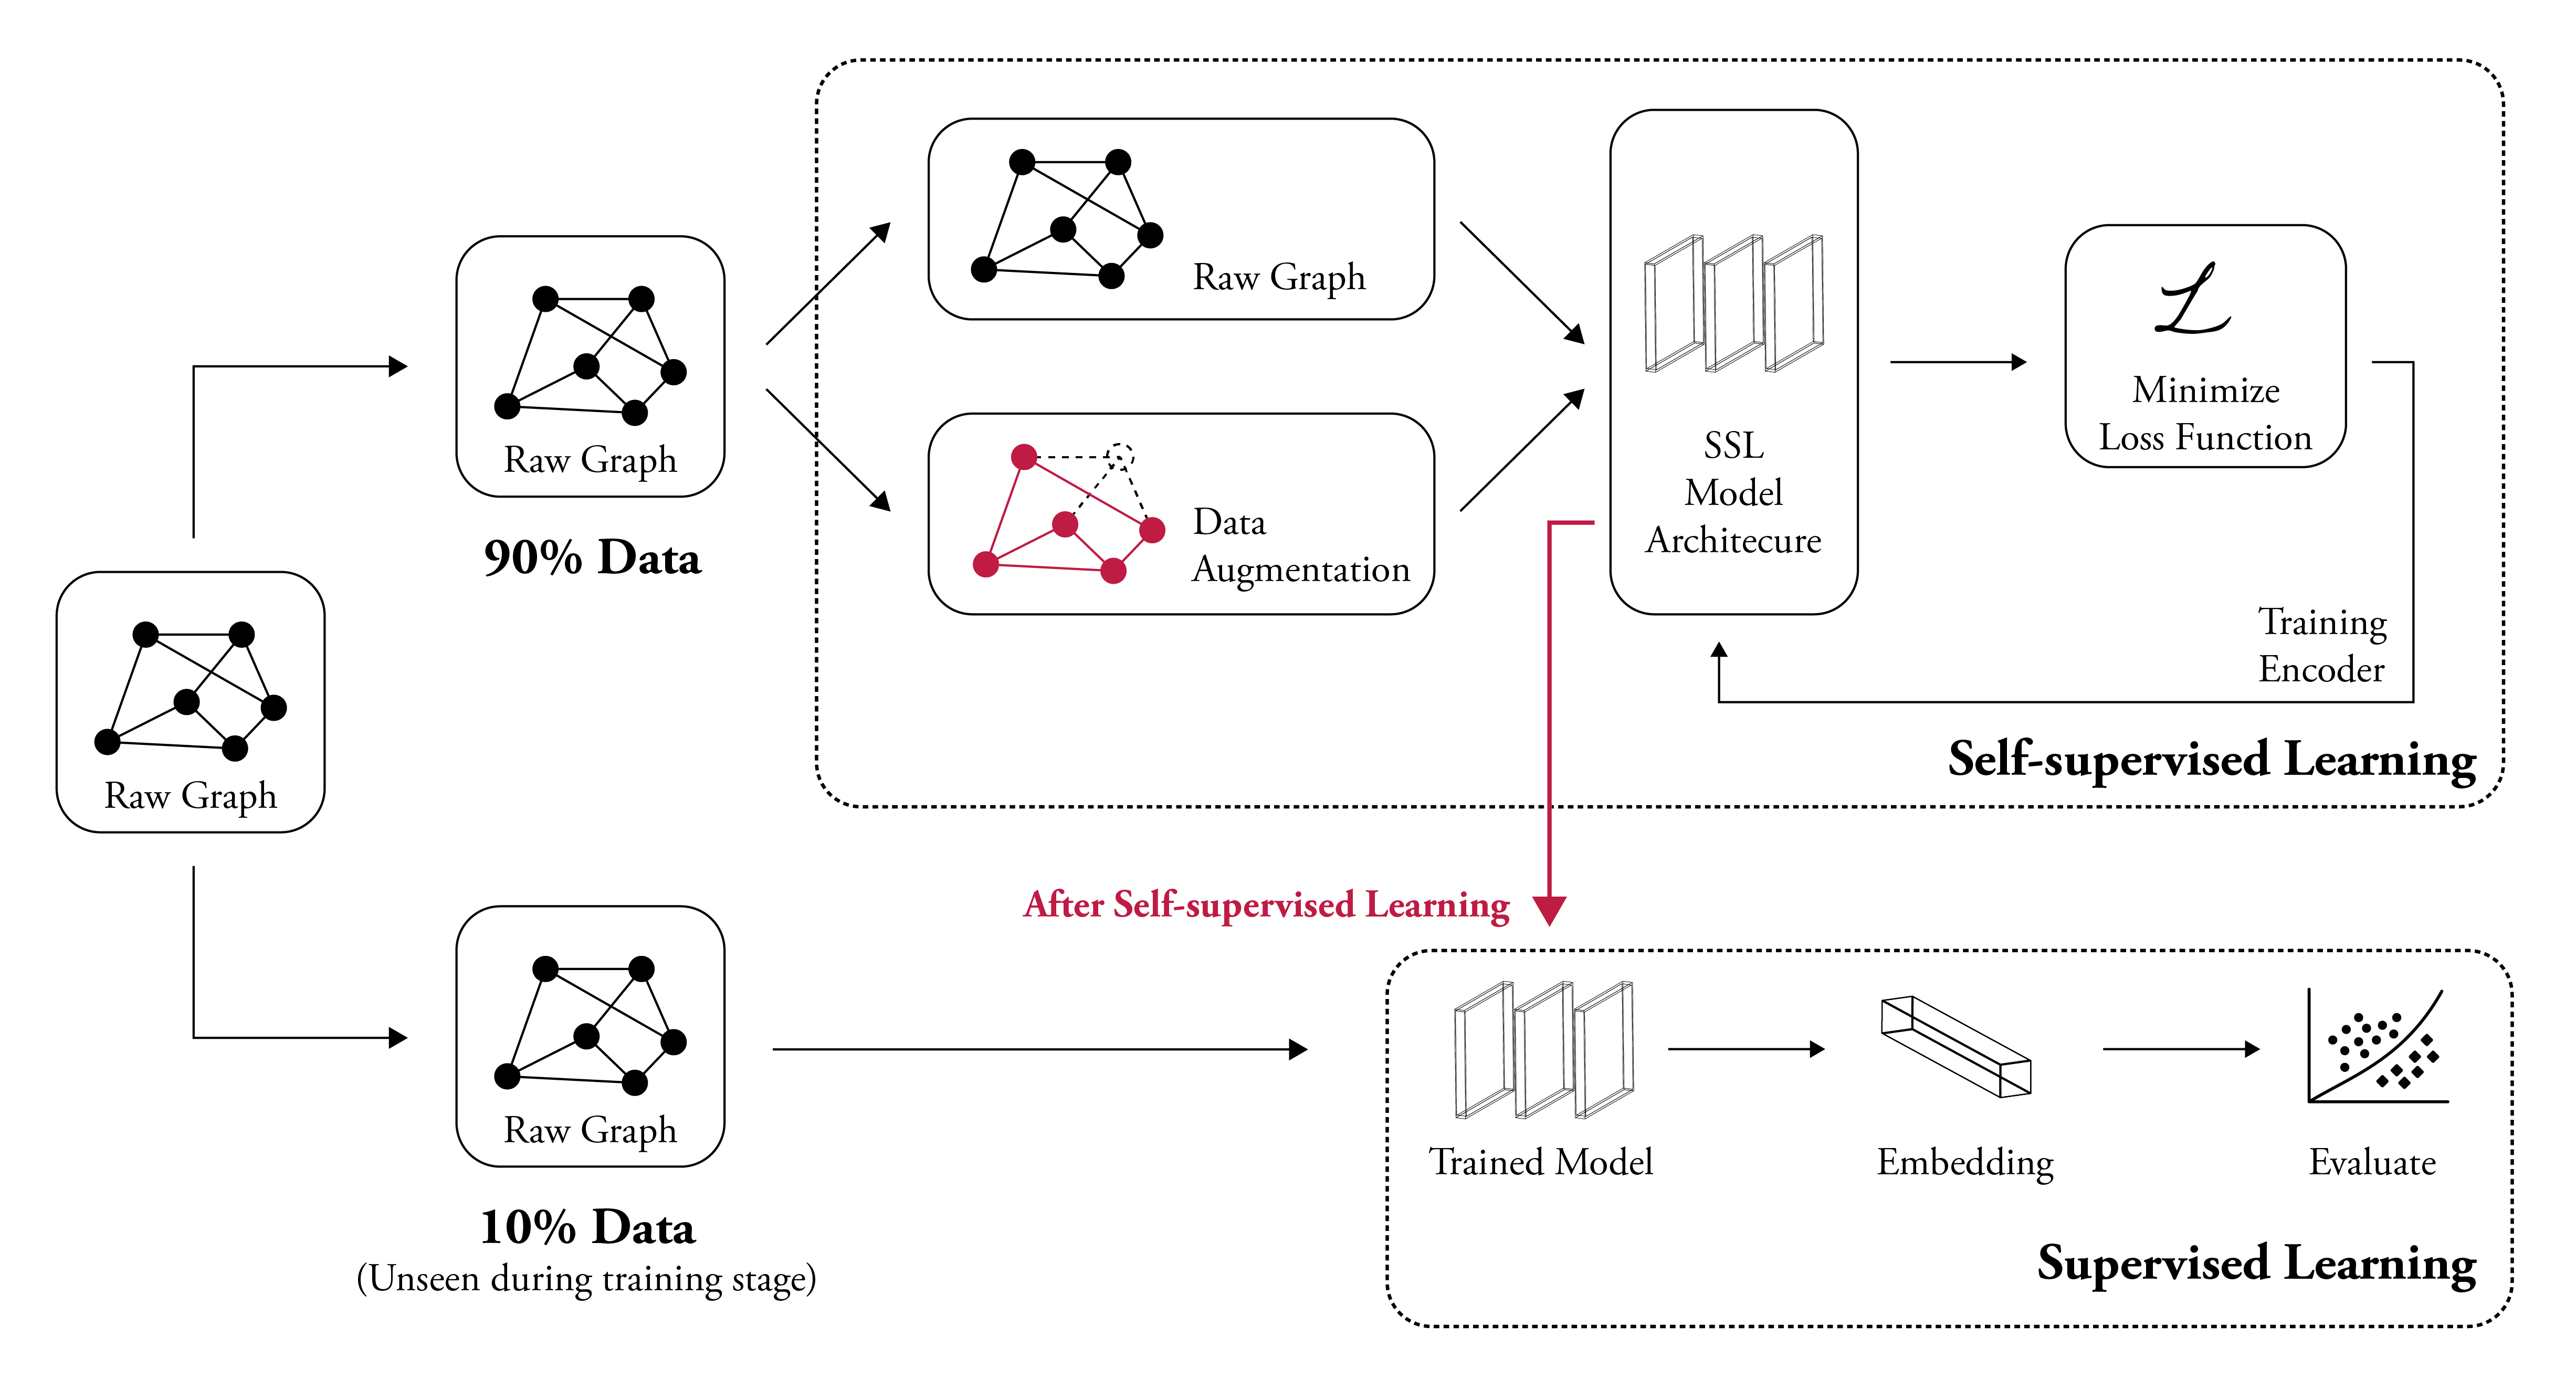
\includegraphics[width=\textwidth]{./figures/guide-02.png}
\caption[Flow diagram of experiments]{\textbf{Flow diagram of experiments.}  The experiment can be roughly separated into two parts: 90\% of the data are used to train an encoder via self-supervised learning, and the other 10\% are used to evaluate the performance of the model via supervised learning. }
\label{fig:exp}
\end{figure}


This thesis comprises five themed chapters. In the next chapter, we will review self-supervised learning and benchmark GNN models, which serve as encoders for extracting features from graph data. Then, we will describe three self-supervised learning methods in Chapter 3 that will be further used to train GNNs on unlabeled data. In Chapter 4, we will evaluate the performance of the three self-supervised learning methods by conducting simulation experiments, where several GNNs will be trained on real-world data under different experiment settings. Finally, we will briefly describe possible future research directions in the last chapter as a conclusion.






% !TeX root = ../main.tex

\chapter{Literature Reviews}

In this chapter, we review recent developments in self-supervised learning and graph neural networks.  



\section{Self-supervised Learning}

Supervised learning is the most widely adopted ML approach for training deep neural networks (DNNs). However, it requires large amounts of labeled data for success. Due to the limited human resources and computing power, it is difficult to obtain large amounts of labeled data. Because of this difficulty, self-supervised learning has received significant attention in recent years. 

Being a branch of unsupervised learning, self-supervised learning trains models by leveraging information from data themselves without guidance from labels or other external information. In image processing or NLP, there is a common situation in which there are large amounts of data but only a small fraction of them are labeled \cite{zhu2021empirical}. 

Several methods based on self-supervised learning have been developed in recent years. In 2018, a memory bank \cite{MemoryBank} structure was introduced into machine learning. Researchers use the convolutional neural network (CNN) backbone to generate high-dimension features of original images, store these features in a memory bank, and then use a non-parametric softmax classifier with NCE loss and proximal regularization to calculate the probability of prediction and train an encoder. This process is regarded as the basis of contrastive learning \cite{hassani2020contrastive}.

%%%%%%%%%%%%%%%%%%%%%%%%%%%%%%%%%%%%%%%%%%%%%%%%%%%%%%%%

Based on the memory bank architecture, MoCo (\textit{Momentum Contrast}) \cite{MoCo, MoCov2} uses a specific momentum-updated encoder, a memory bank, and a dynamic queue used for generating negative samples. MoCo performs the learning procedure by comparing positive and negative sample pairs. MoCo can produce models that outperform supervised models in several ImageNet-related tasks. 

%%%%%%%%%%%%%%%%%%%%%%%%%%%%%%%%%%%%%%%%%%%%%%%%%%%%%%%%

SimCLR (\textit{A Simple Framework for Contrastive Learning of Visual Representations}) \cite{SimCLR, chen2020big} is another self-supervised learning method based on the idea of contrastive learning. SimCLR first applies several data augmentation methods to an image and then inputs a data pair into an encoder to obtain the embedding. The embedding is then mapped to a latent space through a projector. In this latent space, positive and negative sample pairs are compared to train the encoder.


SimCLR can achieve better performance than supervised models in several ImageNet-related tasks. In addition, the authors have proposed several tips to improve the performance of self-supervised learning, including using a larger batch size, a multilayer architecture as the projector, and different types of image data augmentation methods such as Gaussian deblur. 

In MoCo and SimCLR, the distance between each pair of projections is calculated, and similar projections should have a closer distance than the other unrelated pairs. Another method for performing such comparison, known as clustering learning, is to let the encoder group closer projections as a cluster by itself.

%%%%%%%%%%%%%%%%%%%%%%%%%%%%%%%%%%%%%%%%%%%%%%%%%%%%%%%%

DeepCluster \cite{DeepClustering} introduces a clustering module into the latent feature layer. Features generated from input images will be separated into various clusters. After the pseudo-labeling stage, each cluster will be regarded as a unique class. The model will train the encoder via backpropagation.

%%%%%%%%%%%%%%%%%%%%%%%%%%%%%%%%%%%%%%%%%%%%%%%%%%%%%%%%

To prevent mapping all data points to the same cluster, SeLa (\textit{Self Labelling}) \cite{SeLa} adds some constraints on a label by maximizing the information between the label and input data. Furthermore, SeLa uses the Sinkhorn–Knopp algorithm to speed up the self-labeling process and reduce the training time.

%%%%%%%%%%%%%%%%%%%%%%%%%%%%%%%%%%%%%%%%%%%%%%%%%%%%%%%%

SwAV (\textit{Swapping Assignments Between Views}) \cite{SwAV} computes encoded probability by matching projections to prototype clusters. SwAV adopts one's assignment to predict the projection of another by swapping cluster assignments between different images. 

Contrastive and clustering learning are powerful self-supervised learning approaches. However, they require a large number of negative samples to train an encoder. Without negative samples, an encoder can only be trained with positive representation information, causing a trained model to easily converge to a trivial solution or suffer from gradient collapse. 

%%%%%%%%%%%%%%%%%%%%%%%%%%%%%%%%%%%%%%%%%%%%%%%%%%%%%%%%

To tackle this problem, BYOL (\textit{Bootstrap Your Own Latent}) \cite{BYOL} connects a predictor to the projector in the MoCo architecture. The predictor learns by mapping projection from an online network (student encoder) to a target network (teacher encoder, similar to the momentum encoder in MoCo). In addition, only the online network is updated via backpropagation during training. The target network is updated using a stop-gradient mechanism and an exponential average of the online network. In this sense, BYOL can also be regarded as a special type of distillation learning approach. 

%%%%%%%%%%%%%%%%%%%%%%%%%%%%%%%%%%%%%%%%%%%%%%%%%%%%%%%%

Another distillation learning method is called Simsiam (\textit{Simple Siamese Representation Learning}) \cite{Simsiam}. Simsiam is inspired by BYOL, but unlike BYOL, the former simplifies the prototype of the online and target networks by removing the momentum-updated target encoder and connecting the target network directly to the online network. 

%%%%%%%%%%%%%%%%%%%%%%%%%%%%%%%%%%%%%%%%%%%%%%%%%%%%%%%%

Negative samples are not required in distillation learning methods such as BYOL and Simsiam. Instead, they used the predictor and stop-gradient mechanism to train a powerful encoder.

As discussed above, the contrastive, clustering, and distillation learning approaches train an encoder from the sample projection. Barlow Twins \cite{BarlowTwins}, another self-supervised learning method, starts from another perspective. Inspired by neuroscientist H. Barlow's redundancy reduction principle, Barlow Twins uses the embedding without considering negative samples or momentum average. It focuses on training an encoder that can yield data representation without redundant components. Barlow Twins can also achieve good performance on ImageNet-related tasks.

%%%%%%%%%%%%%%%%%%%%%%%%%%%%%%%%%%%%%%%%%%%%%%%%%%%%%%%%

Self-supervised learning has made remarkable progress in recent years. Table \ref{tab:methods} shows the learning approaches and methods to which they belong.



\begin{table}[!htbp]
\centering
\begin{tabular}{c|c}
\toprule

Contrastive Learning & \makecell[l]{Memory Bank (Wu et al., 2018 \cite{MemoryBank})\\Moco (He et al., v1:2019 \cite{MoCo}; v2:2020 \cite{MoCov2}) \\ SimCLR (Chen et al., 2020a \& 2020b \cite{SimCLR, chen2020big})}\\

\midrule

Clustering Learning & \makecell[l]{DeepCluster (Caron et al., 2019 \cite{DeepClustering}) \\ SeLa (Asano et al., 2020 \cite{SeLa}) \\ SwAV (Caron et al., 2020 \cite{SwAV})}\\

\midrule

Distillation Learning& \makecell[l]{BYOL (Grill et al.,2020 \cite{BYOL})\\ Simsiam (Chen \& He, 2020 \cite{Simsiam})}\\

\midrule

Redundancy Reduction& \makecell[l]{Barlow Twins (Zbontar et al., 2021 \cite{BarlowTwins})}\\

\bottomrule
\end{tabular}
\vspace{0.5cm}
\caption[Approaches of self-supervised learning]{\textbf{Approaches of self-supervised learning.}}

		\label{tab:methods}

	\end{table}

%%%%%%%%%%%%%%%%%%%%%%%%%%%%%%%%%%%%%%%%%%%%%%%%%%%%%%%%
%%%%%%%%%%%%%%%%%%%%%%%%%%%%%%%%%%%%%%%%%%%%%%%%%%%%%%%%
%%%%%%%%%%%%%%%%%%%%%%%%%%%%%%%%%%%%%%%%%%%%%%%%%%%%%%%%

\section{Graph Neural Networks (GNN)}

A graph is a type of data structure for non-tablize information. It is commonly seen in knowledge graph \cite{knowledge}, social network \cite{social}, recommendation system \cite{recommender}, combinatorial optimization \cite{combinatorial}, particle simulation \cite{particle}, molecule discovery \cite{antibiotic}, and many other machine learning related tasks. Owing to its specific structure, we can use a neighborhood aggregation and message passing scheme to capture information within nodes' neighborhoods, which can preserve the relationship between each node and edge rather than use the table format \cite{comprehensive}..

Consider a graph $\mathcal{G} = (\mathcal{V},\mathcal{E})$, where $\mathcal{V}$ denotes a set of nodes and $\mathcal{E}$ denotes a set of edges. Let $\mathcal{N}_{u}$ denote a node set of nodes adjacent to node $u\in \mathcal{V}$. We can obtain the $\mathbf{h}_{u}^{(k)}$, the feature vector of node $u$ at the $k$th layer, via the following operators:

\begin{equation}
\mathbf{h}_{u}^{(k)}=\text{COMBINE}^{(k)}\Big(\mathbf{h}_{u}^{(k-1)},\mathbf{a}_{u}^{(k)}\Big),
\end{equation}

where

\begin{equation}
\mathbf{a}_{u}^{(k)}=\text{AGGREGATE}^{(k)}\Big(\{\mathbf{h}_{v}^{(k-1)}, \forall v\in\mathcal{N}_{u}\}\Big).
\end{equation}

During the iteration of neural networks, the $\text{AGGREGATE}(\cdot)$ operator generates aggregation message $\mathbf{a}_{u}^{(k)}$ based on the aggregated information of adjacent nodes set $\mathcal{N}_{u}$. Subsequently, the aggregation message of node $u$ and the feature of previous $k-1$th layer $\mathbf{h}_{u}^{(k-1)}$ will be combined to generate the updated feature in the latest $k$th layer, $\mathbf{h}_{u}^{(k)}$, through the $\text{COMBINE}(\cdot)$ operator.

After generating each feature of nodes using a $K$-layer GNN, we can use a $\text{READOUT}(\cdot)$ operator to obtain the entire graph embedding $\mathbf{h}$ of $\mathcal{G}$:

\begin{equation}
\mathbf{h}=\text{READOUT}\Big(\{\mathbf{h}_{u}^{(K)}, \forall u\in\mathcal{V}\}\Big).
\end{equation}

Based on the use of different $\text{COMBINE}(\cdot)$ and $\text{AGGREGATE}(\cdot)$ operators, several architectures for encoding graph data have been proposed. For example, GraphSAGE \cite{GraphSAGE} uses element-wise max-pooling $\text{MAX}(\cdot)$ with a non-linear function $\sigma(\cdot)$, such as ReLu or sigmoid function, as the $\text{AGGREGATE}(\cdot)$ operator and concatenates the aggregation vector and $k-1$th feature vector to obtain the updating feature:

\begin{equation}
\textbf{a}_{u}^{(k)}={\text{MAX}\Big(\Big\{\sigma(\Theta^{(k)}\cdot\textbf{h}_{v}^{(k-1)}),\forall v\in\mathcal{N}_{u}\Big\}\Big)},
\end{equation}

\begin{equation}
\mathbf{h}_{u}^{(k)}={\text{CONCAT}\Big(\mathbf{h}_{u}^{(k-1)}, \textbf{a}_{u}^{(k)}\Big)}.
\end{equation}

where $\Theta^{(k)}$ is a learnable weight matrix.

By contrast, Graph Convolutional Networks (GCN) \cite{GCN} use element-wise mean pooling $\text{MEAN}(\cdot)$ for information propagation, and the $\text{AGGREGATE}(\cdot)$ and $\text{COMBINE}(\cdot)$ functions are integrated as follows:

\begin{equation}
\mathbf{h}_{u}^{(k)}=\text{ReLu}\Big(\Theta^{(k)}\cdot\text{MEAN}\Big\{\mathbf{h}_{v}^{(k-1}, \forall v\in\mathcal{N}_{u}\cup\{u\}\Big\}\Big).
\end{equation}

Furthermore, Graph Isomorphism Network (GIN) \cite{GIN} use multilayer perceptrons (MLPs) for information propagation because they can represent a good function composition. The iteration function can be represented as

\begin{equation}
\textbf{a}_{u}^{(k)}=\Big(\sum_{v\in\mathcal{N}_{u}}\mathbf{h}_{v}^{(k-1)}\Big),
\end{equation}

\begin{equation}
\mathbf{h}_{u}^{(k)}=\text{MLP}\Big((1+\epsilon^{(k)})\cdot\mathbf{h}_{u}^{(k-1)}+\textbf{a}_{u}^{(k)}\Big),
\end{equation}

\begin{equation}
\textbf{h} = \text{CONCAT}\Big( \mathbf{h}_{u}^{(K)}, \forall u \in \mathcal{V} \Big).
\end{equation}

where $\epsilon$ can be a learnable parameter or a fixed scalar. 

In this thesis, we will choose Graph Isomorphism Network as the main encoder for encoding graph data. The details are presented in Table  \ref{tab:expfactor}.



\section{Discussion}

In this chapter, we have described the basic idea of self-supervised learning. Furthermore, we have reviewed several benchmark GNN models, including GraphSAGE, Graph Convolutional Networks, and Graph Isomorphism Networks. 

In the next chapter, we will present more details on model training, including the datasets, data augmentation techniques, and the three self-supervised learning methods that we will use to train those GNNs on unlabeled data.











% !TeX root = ../main.tex

\chapter{Methodology}

Many factors can influence model performance, including encoder structure, depth and width of layers, and batch size. This thesis investigates the effects of these factors on model performance, particularly the performance of models trained on graph data via self-supervised learning. 

Next, we introduce our experiment settings, including the datasets, data augmentation methods, hyperparameters in the training procedure, and self-supervised learning methods we use for model training.

\section{Dataset}

We mainly use the following datasets for model training: MUTAG, NCI1, PROTEINS, and DD. These datasets are collected by TUDataset \cite{tudataset} and are widely used in graph representation learning for evaluating model performance \cite{benchmarking}. 

These datasets contain graph data falling into two categories: chemical molecules and bioinformatics. In MUTAG \cite{mutag} and NCI1 \cite{nci1}, each graph is used to represent a chemical compound or molecule. Each node represents an atom, and each edge represents a chemical bond connecting two nodes. Both datasets are collected for binary graph classification tasks encoded by a one-hot encoding. The prediction task of MUTAG is to predict the mutagenicity of \textit{Salmonella typhimurium}, and the task of NCI1 is to determine whether a chemical compound is positive or negative for cell lung cancer.

On the other hand, in PROTEINS \cite{proteins} and DD \cite{proteins}, each graph is used to represent a protein structure. Each node represents an amino acid, and two nodes are connected by an edge if their distance is less than 6 angstroms apart. The prediction tasks of both datasets are to classify protein structures as enzymes or non-enzymes.

Table \ref{tab:dataset} provides the statistical details of these datasets.


\begin{table}[!htbp]
\centering
\begin{tabular}{l|c|c|c|c|c}
\toprule
Dataset & Category & \# Graphs & \# Classes & Avg. Nodes & Avg. Edges \\ 
\midrule
MUTAG \cite{mutag} & Molecules & 188 & 	2	&17.93&	19.79 \\
NCI1 \cite{nci1} & Molecules & 4110	&2&	29.87&	32.30 \\
\midrule
PROTEINS \cite{proteins} & Bioinformatics & 1113	&2	&39.06&	72.82 \\
DD \cite{proteins} & Bioinformatics & 1178&	2	&284.32&	715.66 \\
\bottomrule
\end{tabular}
\vspace{0.5cm}
\caption[Statistics of datasets]{\textbf{Statistics of datasets.} Incidentally, these datasets are collected for graph classification tasks. }
		\label{tab:dataset}
	\end{table}
	
	
%%%%%%%%%%%%%%%%%%%%%%%%%%%%%%%%%%%%%%%%%%%%%%%%%%%%%%%%%%%%%%%%
%%%%%%%%%%%%%%%%%%%%%%%%%%%%%%%%%%%%%%%%%%%%%%%%%%%%%%%%%%%%%%%%
%%%%%%%%%%%%%%%%%%%%%%%%%%%%%%%%%%%%%%%%%%%%%%%%%%%%%%%%%%%%%%%%


\section{Data Augmentation}

Self-supervised learning heavily relies on data augmentation for model training \cite{ding2022data, zhao2022graph}. Designing a robust and useful augmentation method is an imperative task in the preprocessing stage. Unlike image data, which can be augmented using methods such as random cropping, blurring, or rotation, graph data are subject to different mechanisms for augmentation. Based on GraphCL, we adopt the following four methods for augmenting our graph data:

\textbf{\uppercase{attribute masking.}} This operator replaces an original attribute with a random value generated by a normal distribution. Generally, some nodes have unique attributes. For example, an atom has its chemical property. We expect that a small change in a few nodes' attributes should not affect the information of the graph. 
		
\textbf{\uppercase{node dropping.}} This operator randomly drops some nodes and their linked edges that connect to other nodes. For example, if we set the augmentation ratio to $0.3$, a total of 30\% of the nodes and their connected edges will be dropped. Despite a few nodes being ignored, we expect the hidden information and features of the graph not to be significantly affected.	

\textbf{\uppercase{edge perturbation.}} Similar to the \uppercase{node dropping} operator, this operator randomly adds or deletes an edge based on a specific ratio. We expect that when a few edges between nodes in a graph are perturbed, the hidden property of the graph will be unaffected. 

\textbf{\uppercase{subgraph.}} This operator randomly samples a subgraph from the local part of the raw graph. In general, we expect the information in the graph to be preserved in its partial structure. 

The illustrations for our data augmentation procedures are shown in Figure \ref{fig:aug}, where the red parts drawn in graphs are the output of data augmentation.


\begin{figure}[!htbp]
\centering
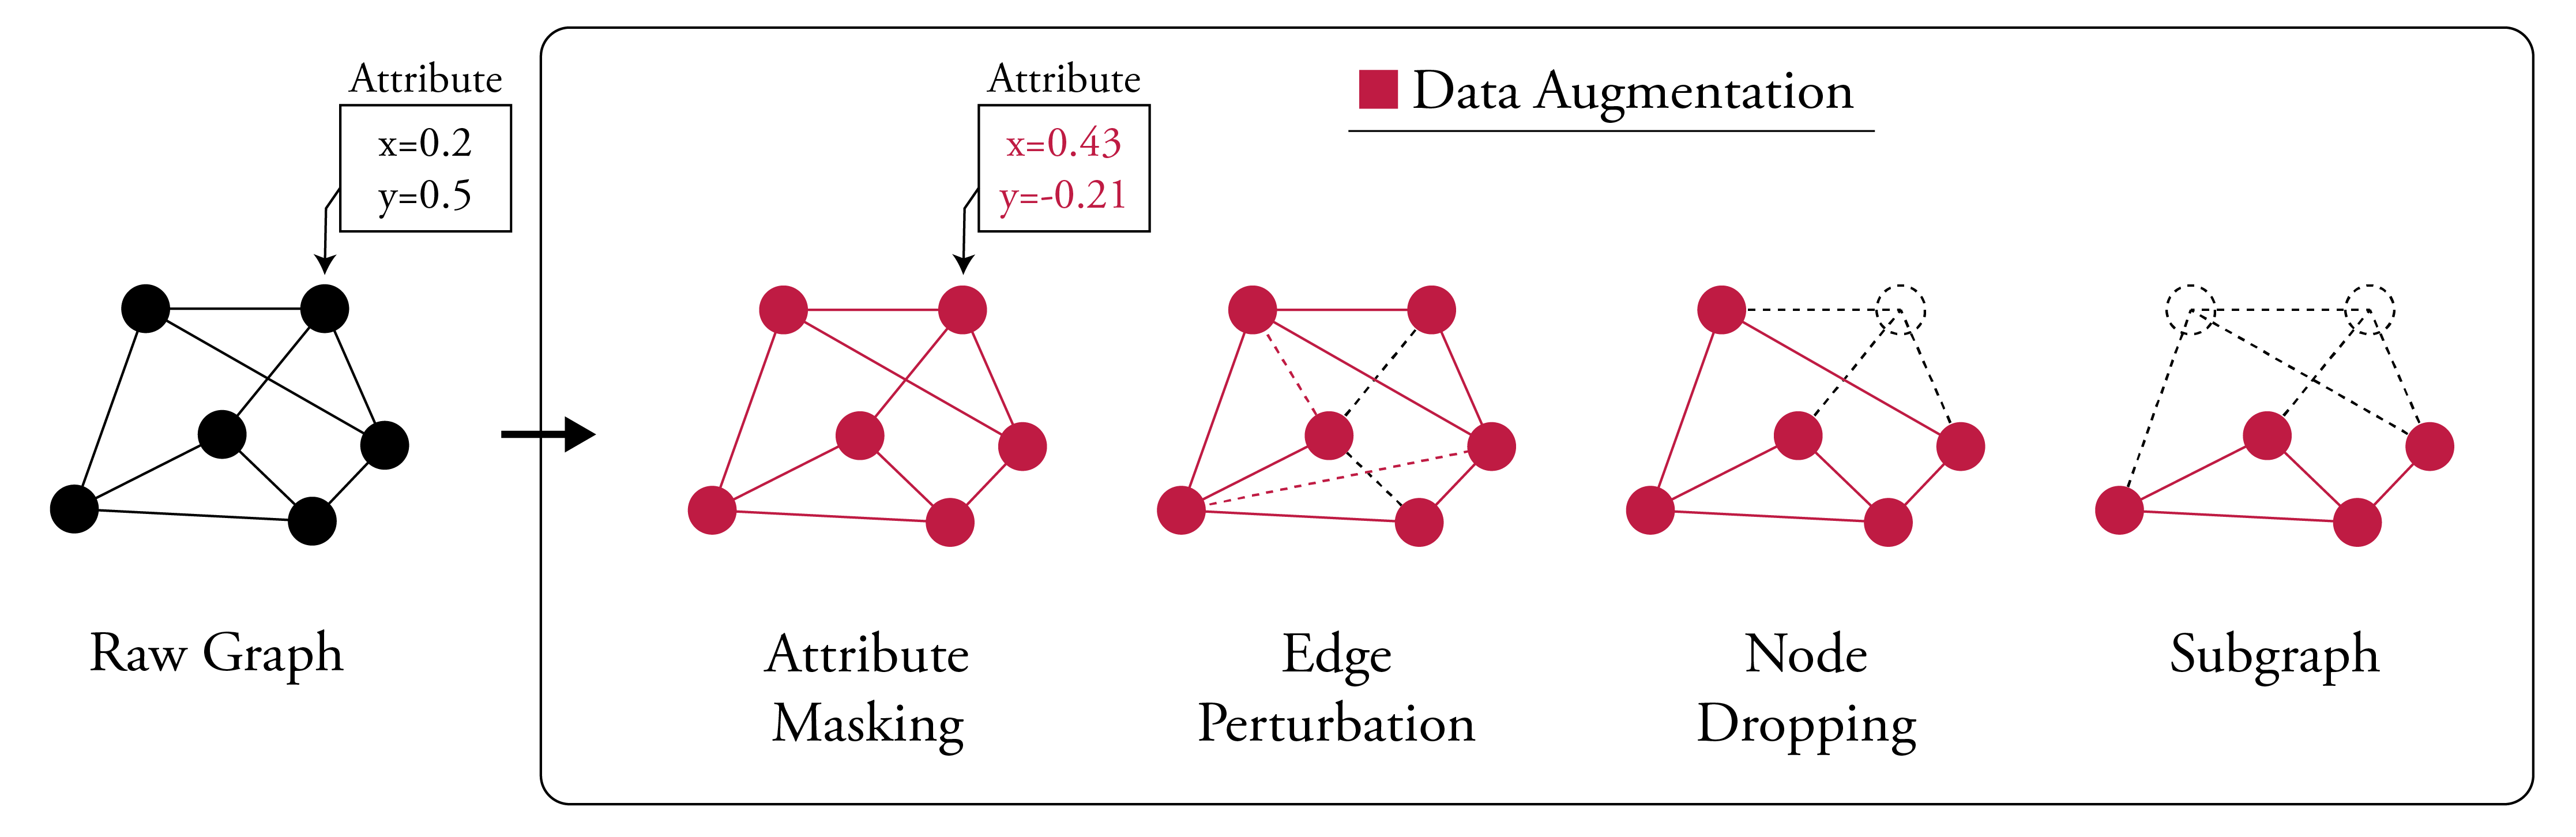
\includegraphics[width=1\textwidth]{./figures/data_augmetation_aka.png}
\vspace{0.5cm}
\caption[Illustrations of augmentation operators]{\textbf{Illustrations of augmentation operators.} Compared with the leftmost raw graph, the red parts drawn in the graphs are the output after data augmentation. The augmented ratio is set to 0.3.}
\label{fig:aug}
\end{figure}


%%%%%%%%%%%%%%%%%%%%%%%%%%%%%%%%%%%%%%%%%%%%%%%%%%%%%%%%%%%%%%%%
%%%%%%%%%%%%%%%%%%%%%%%%%%%%%%%%%%%%%%%%%%%%%%%%%%%%%%%%%%%%%%%%
%%%%%%%%%%%%%%%%%%%%%%%%%%%%%%%%%%%%%%%%%%%%%%%%%%%%%%%%%%%%%%%%



\section{Experiment Factor}

To compare the performance of different models trained on graph data, we conducted a series of experiments with varying experiment factors.

We adopted the three self-supervised learning methods, SimCLR, Simsiam, and Barlow Twins, along with the four data augmentations described in Section 3.2, to train our encoders. We set the batch size equal to 64 and 256 (for models trained on the DD dataset, we set the batch size equal to 64 and 128) and the dimension of the hidden space equal to 64 and 512. 

In addition, because the depth of an encoder is a key factor in self-supervised learning, we adopted the monolayer, bilayer, and trilayer architectures for Graph Isomorphism Networks. Because of these experiment settings, there are 144 experiments for each of the four datasets.

These experiment factors are listed in Table \ref{tab:expfactor}. Each experiment was repeated five times to obtain an average result and standard deviation.


\begin{table}[!htbp]
\centering
\begin{tabular}{r|l}
\toprule
Self-Supervised Approach & \makecell[l]{
~~\llap{\textbullet}~~SimCLR (See Section 3.4 and Figure \ref{fig:arch-simclr}) \\
~~\llap{\textbullet}~~Simsiam (See Section 3.5 and Figure \ref{fig:arch-simsiam})\\
~~\llap{\textbullet}~~Barlow Twins (See Section 3.6 and Figure \ref{fig:arch-bt})} \\
\midrule
Data Augmentation & \makecell[l]{
~~\llap{\textbullet}~~\uppercase{attribute masking}\\
~~\llap{\textbullet}~~\uppercase{edge perturbation} \\
~~\llap{\textbullet}~~\uppercase{node droppping}\\
~~\llap{\textbullet}~~\uppercase{subgraph}\\
~~\llap{\textbullet}~~with ratio 0.3} \\
% \midrule
% Augmentation Ratio & 0.3 \\
\midrule
Mini-batch Size & \makecell[l]{
~~\llap{\textbullet}~~for MUTAG, PROTEINS, NCCI1: 64, 256\\
~~\llap{\textbullet}~~for DD: 64, 128}\\
\midrule
Hidden Dimension & 64, 512\\
\midrule
Encoder & \makecell[l]{~~\llap{\textbullet}~~Encoder Type: Graph Isomorphism Network (GIN)\\
~~\llap{\textbullet}~~Number of Layer: 1 (monolayer), 2 (bilayer), 3 (trilayer)} \\
\midrule
Number of Projector Layer & 3 (trilayer)\\
\midrule
Learning Rate & \makecell[l]{~~\llap{\textbullet}~~0.01\\
~~\llap{\textbullet}~~for Simsiam, with stop-gradient mechanism}\\
\midrule
Epoch  & 200\\
\midrule
Data Proportion & \makecell[l]{
~~\llap{\textbullet}~~ 90\% used in self-supervised for training stage\\
~~\llap{\textbullet}~~ 10\% used in supervised for validation and testing stage}
\\


\bottomrule
\end{tabular}
\vspace{0.5cm}
\caption[Detail of experiment factors]{\textbf{Detail of Experiment factors.} The use of different independent and control variables to observe the effect of each factor resulted in 144 experiments being conducted.}
		\label{tab:expfactor}
	\end{table}


%%%%%%%%%%%%%%%%%%%%%%%%%%%%%%%%%%%%%%%%%%%%%%%%%%%%%%%%%%%%%%%%
%%%%%%%%%%%%%%%%%%%%%%%%%%%%%%%%%%%%%%%%%%%%%%%%%%%%%%%%%%%%%%%%
%%%%%%%%%%%%%%%%%%%%%%%%%%%%%%%%%%%%%%%%%%%%%%%%%%%%%%%%%%%%%%%%


\section{Contrastive Learning: SimCLR}

Let $\mathbf{x}$ denote the raw data. In SimCLR, we can obtain $\mathbf{x}$'s embedding $\mathbf{h}$ using an encoder $\phi(\cdot)$ and obtain its projection $\mathbf{z}$ through a projector $\theta(\cdot)$. Similarly, we can obtain the augmented embedding $\mathbf{h}^{*}$ and augmented projection $\mathbf{z}^{*}$ using the augmented data $\mathbf{x}^{*}$, where $\mathbf{x}^{*} = \text{AugOperator}(\mathbf{x})$. Mathematically, we can express $\mathbf{h}$ and $\mathbf{z}$ by

\begin{equation}
\mathbf{h}=\phi(\mathbf{x}),
\end{equation}

\begin{equation}
\mathbf{z}=\theta(\mathbf{h})=\theta\Big(\phi(\mathbf{x})\Big), 
\end{equation}

respectively. According to empirical experiments and observation, a projector can make representation more flexible and improve prediction effects.

The loss function used by SimCLR is the NT-Xent loss (normalized temperature-scaled cross entropy loss). For a positive pair of representations $(\mathbf{z},\mathbf{z}^{*})$, the loss function is defined as

\begin{equation}
\mathit{Loss}=-\log\frac{\exp\big(\textbf{sim}(\mathbf{z},\mathbf{z}^{*})/\tau\big)}{\sum^{N}_{\mathbf{z}^{'}\neq\mathbf{z}}\exp\big(\textbf{sim}(\mathbf{z},\mathbf{z}^{'})/\tau)\big)},
\end{equation}

where

\begin{equation}
\textbf{sim}(\mathbf{a},\mathbf{b})=\frac{\mathbf{a}^{\intercal}\mathbf{b}}{\|\mathbf{a}\|_2\|\mathbf{b}\|_2}
\end{equation}

where $\tau$ denotes the trainable temperature parameter and $\textbf{sim}(\mathbf{a},\mathbf{b})$ denotes the $\mathit{l}_2$ normalized cosine similarity between two vectors $\mathbf{a}$ and $\mathbf{b}$. Throughout the experiments, we set $\tau = 0.2$. Notice that the negative representation $\mathbf{z}^{'}$ is generated from the other $N-1$ samples, and the gradient is updated using both the raw and augmented data.

\begin{figure}[!htbp]
% \centering
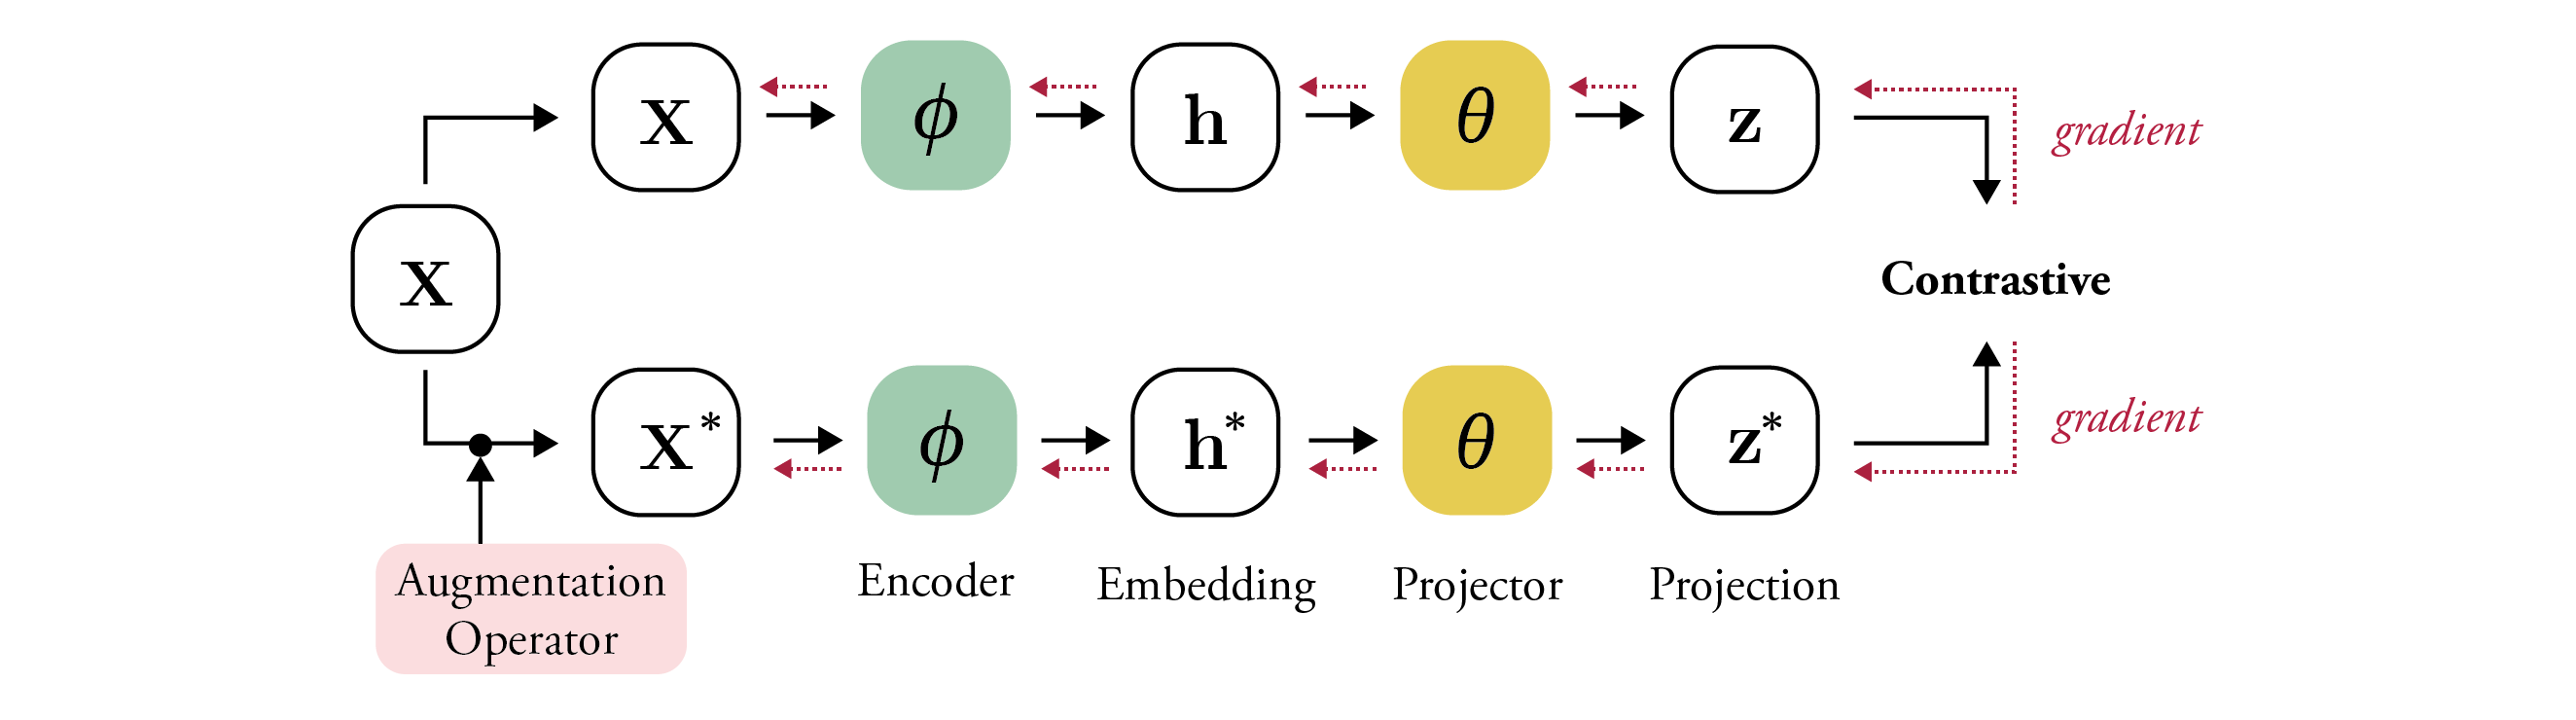
\includegraphics[width=1\textwidth]{./figures/model3_simclr.png}
\vspace{0.5cm}
\caption[Architecture of SimCLR models]{\textbf{Architecture of SimCLR models.} The encoder will learn from the projection of raw and augmented data via NT-Xent loss. According to empirical experiments and observation, a projector can make representation more flexible and improve prediction effects.}
\label{fig:arch-simclr}
\end{figure}


%%%%%%%%%%%%%%%%%%%%%%%%%%%%%%%%%%%%%%%%%%%%%%%%%%%%%%%%%%%%%%%%
%%%%%%%%%%%%%%%%%%%%%%%%%%%%%%%%%%%%%%%%%%%%%%%%%%%%%%%%%%%%%%%%
%%%%%%%%%%%%%%%%%%%%%%%%%%%%%%%%%%%%%%%%%%%%%%%%%%%%%%%%%%%%%%%%


\section{Distillation Learning: Simsiam}

In Simsiam, we use an encoder $\phi(\cdot)$ and a projector $\theta(\cdot)$ to obtain the embedding and projection of the raw data $\mathbf{x}$ and the augmented data $\mathbf{x}^{*}$. Moreover, Simsiam introduces a predictor $\psi(\cdot)$ that generates the prediction $\textbf{p}$ via

\begin{equation}
\textbf{p}=\psi(\textbf{z})=\psi(\theta(\mathbf{h}))=\psi\Big(\theta(\phi(\textbf{x}))\Big).\
\end{equation}

The loss function follows the cosine similarity between pairs $(\textbf{z}^{*},\textbf{p})$ and $(\textbf{z},\textbf{p}^{*})$. It is defined by

\begin{equation}
\begin{split}
\mathit{Loss}&=-\frac{1}{2}\sum^{N}_{\text{Dataset}}\Big(\textbf{sim}(\textbf{z}^{*},\textbf{p})+\textbf{sim}(\textbf{z},\textbf{p}^{*})\Big)\\&=-\frac{1}{2}\sum^{N}_{\text{Dataset}}\Big(\frac{(\mathbf{z}^{*})^{\intercal}\mathbf{p}}{\|\mathbf{z}^{*}\|_{2}\|\mathbf{p}\|_{2}}+\frac{\mathbf{z}^{\intercal}\mathbf{p}^{*}}{\|\mathbf{z}\|_{2}\|\mathbf{p}^{*}\|_{2}} \Big).
\end{split}
\end{equation}

To prevent gradient collapse, $\textbf{z}$ and $\textbf{z}^{*}$, the representations produced by the target network, are treated as constants in the training stage. They are subject to the stop-gradient operator when computing the gradient of the loss function. Only $\mathbf{p}$ and $\mathbf{p}^{*}$, the representations produced by the online network, are updated.

As shown in Figure \ref{fig:arch-simsiam}, to calculate the similarity of $(\textbf{z}^{*},\textbf{p})$, Simsiam feeds raw graphs to the online network and augmented graphs to the target network. Thus, only the gradient in the online network is updated via backpropagation. Similarly, when Simsiam calculates the similarity of $(\textbf{z},\textbf{p}^{*})$, it will send raw graphs to the target network and send augmented graphs to the online network.


\begin{figure}[!htbp]
% \centering
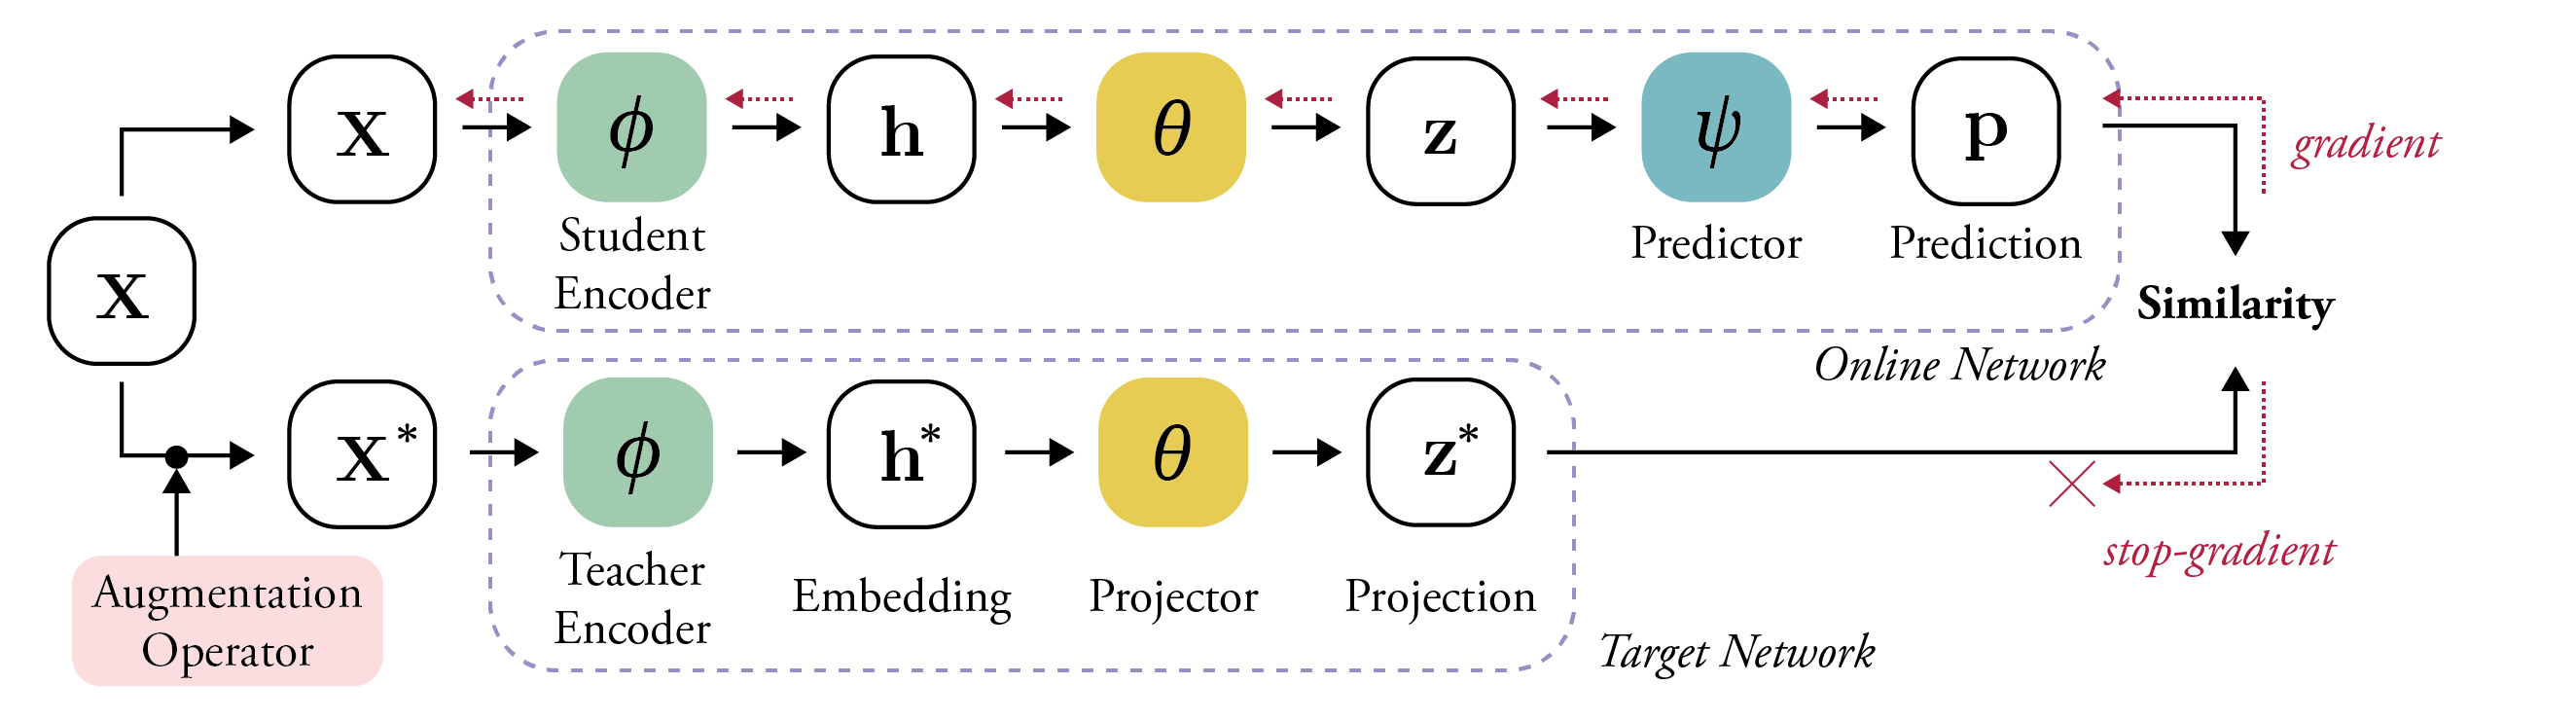
\includegraphics[width=1\textwidth]{./figures/model3_simsiam.png}
\vspace{0.5cm}
\caption[Architecture of Simsiam models]{\textbf{Architecture of Simsiam models.} For example, to calculate the similarity of $(\textbf{z}^{*},\textbf{p})$, Simsiam feeds raw graphs to the online network and augmented graphs to the target network. Only the gradient in the online network is updated via backpropagation.}
\label{fig:arch-simsiam}
\end{figure}


%%%%%%%%%%%%%%%%%%%%%%%%%%%%%%%%%%%%%%%%%%%%%%%%%%%%%%%%%%%%%%%%
%%%%%%%%%%%%%%%%%%%%%%%%%%%%%%%%%%%%%%%%%%%%%%%%%%%%%%%%%%%%%%%%
%%%%%%%%%%%%%%%%%%%%%%%%%%%%%%%%%%%%%%%%%%%%%%%%%%%%%%%%%%%%%%%%


\section{Redundancy Reduction: Barlow Twins}

Compared with Simsiam, which uses the projection–prediction pair $\textbf{z}$ and $\textbf{p}^{*}$, Barlow Twins directly uses the embedding pair for comparison. To calculate the loss function, Barlow Twins \cite{bielak2021graph} computes the cross-correlation matrix $\mathcal{C}$ between the outputs of two identical networks along the batch dimension. The $(i,j)$th element of the correlation matrix $\mathcal{C}$ is defined by

\begin{equation}
\mathcal{C}_{ij}=\frac{\sum_b\big((\tilde{\textbf{h}_\textbf{x}})_{b,i}\big)\cdot\big(\tilde{(\textbf{h}_\textbf{x}^{*}})_{b,j}\big)}{\sqrt{\sum_b\big(\tilde{(\textbf{h}_\textbf{x}})_{b,i}\big)}\cdot\sqrt{\sum_b\big(\tilde{(\textbf{h}_\textbf{x}^{*}})_{b,j}\big)}}.
\end{equation}

where $\tilde{\textbf{h}}$ denotes the normalized embedding of $\textbf{h}$ and $\mathcal{C}_{ij}$ should be between $1$ (perfect correlation) and $-1$ (perfect anticorrelation). If two identical networks are the same, known as perfect correlation, the correlation matrix $\mathcal{C}$ should be a diagonal matrix with $1$, a.k.a. an identity matrix $\mathcal{I}$. 

A good encoder should recognize augmentation data as having the same label as raw data. To train this encoder to distinguish a raw graph from an augmented graph and other irrelevant graphs, the loss function is divided into two parts, namely, the invariance term and redundancy reduction term, which are defined by

\begin{equation}
\mathit{Loss}=\underbrace{\sum_i(1-\mathcal{C}_{ii})^2}_{\text{invariance term}}+\lambda\underbrace{\Big(\sum_i\sum_{i\neq j}\mathcal{C}_{ij}^2\Big)}_{\text{{redundancy reduction  term}}},
\end{equation}

respectively. Here, $\lambda$ is a positive constant used to trade off the importance of the invariance term and redundancy reduction term of the loss. 

\begin{figure}[!htbp]
% \centering
{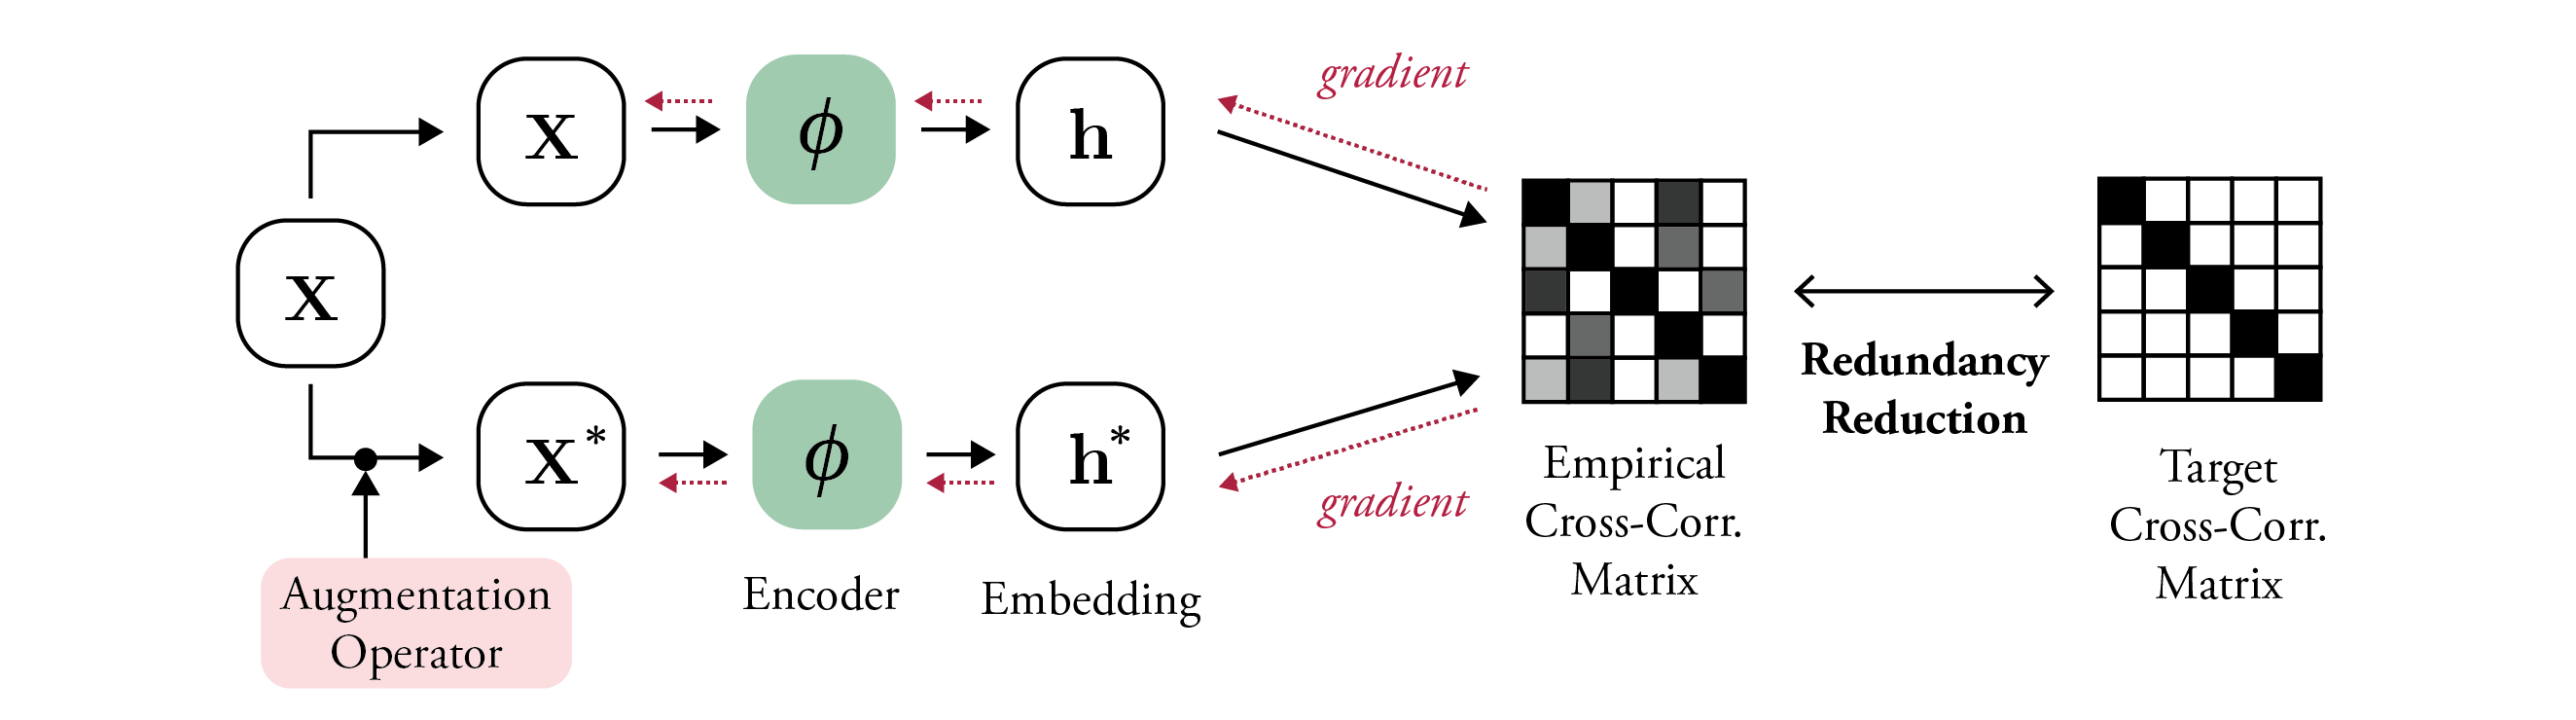
\includegraphics[width=1\textwidth]{./figures/model3_barlowtwins.png}}
\vspace{0.5cm}
\caption[Architecture of Barlow Twins models]{\textbf{Architecture of Barlow Twins models.} The target of an encoder is to classify the embeddings of raw and augmented data as the same label, where the correlation matrix $\mathcal{C}$ of embeddings should be an identity matrix $\mathcal{I}$.}
\label{fig:arch-bt}
\end{figure}


\section{Discussion}

In this chapter, we have described four benchmarks that will be used to train the GNNs. We also have described the data augmentation techniques used in model training. Furthermore, we have discussed the three self-supervised learning methods, SimCLR, Simsiam, and Barlow Twins, that will be used to train the GNNs on unlabeled data: contrastive learning, distillation learning, and dimension reduction approach, respectively. 

In the next chapter, we will evaluate the performance of the three self-supervised learning methods by conducting simulation experiments on the four datasets.

% !TeX root = ../main.tex

\chapter{Results and Discussion}

In this chapter, we will discuss the results of the simulation experiments we described in Chapter 3. Table \ref{tab:result} shows the best results from the 144 experiments on the test dataset between these three learning approaches.

The complete experiment results and a link to the source code can be found in Appendix A. 

\begin{table}[!htbp]
\centering
\begin{tabular}{l|ll|ll}
\toprule
\multicolumn{1}{c|}{}       & \multicolumn{2}{c|}{Molecular Dataset}                & \multicolumn{2}{c}{Bioinformatics Dataset}           \\ \cline{2-5} 
\multicolumn{1}{c|}{Method} & \multicolumn{1}{c}{MUTAG} & \multicolumn{1}{c|}{NCI1} & \multicolumn{1}{c}{DD} & \multicolumn{1}{c}{PROTEINS} \\ \midrule
(1)\,10$\%$ SimCLR                 & 100.0$\pm$0.00             & 74.47$\pm$ 1.45            & 84.36$\pm$4.02           & 76.88$\pm$2.45                \\
(2)\,10$\%$ Barlow Twins           & 94.00$\pm$3.54              & 72.12$\pm$0.82              & 79.94$\pm$2.99           & 83.20$\pm$1.31                \\
(3)\,10$\%$ Simsiam                & 95.00$\pm$0.00              & 73.70$\pm$0.38              & 78.21$\pm$2.76           & 75.29$\pm$2.10                \\ \midrule
(4)\,10$\%$ baseline               & \multicolumn{1}{c}{-}     & 73.72$\pm$0.24              & 73.56$\pm$0.41           & 70.40$\pm$1.54                \\
(5)\,10$\%$ Aug.                   & \multicolumn{1}{c}{-}                         & 73.59$\pm$0.32              & 74.30$\pm$0.81           & 70.29$\pm$0.64                \\
(6)\,10$\%$ GAE                    & \multicolumn{1}{c}{-}                         & 74.36$\pm$0.24              & 74.54$\pm$0.68           & 70.51$\pm$0.17                \\
(7)\,10$\%$ Infomax                & \multicolumn{1}{c}{-}                        & 74.86$\pm$0.26              & 75.78$\pm$0.34           & 72.27$\pm$0.40  
\\
\bottomrule
\end{tabular}
\vspace{0.5cm}
\caption[A summary of experimental results in three learning approaches]{\textbf{A summary of experimental results for three learning approaches.} Each value in the table represents the best average of accuracy (unit: percentage) and the standard deviation in the testing stage. Results (1)–(3) are obtained from our experiments, and for Results (4)–(7), refer to You et al. \cite{GraphCL}}
		\label{tab:result}
\end{table}


\section{Batch size's effects on SimCLR are not apparent}

The authors of SimCLR \cite{SimCLR} pointed out that contrastive learning benefits more from a larger batch size and longer training time. They used different batch sizes, 256, 512, 1024, 2048, 4096, and 8192, to train a ResNet-50 model. They found that these batch sizes are positively correlated with the model's performance, i.e., the larger the batch size, the better the performance of the model. This concept inspires subsequent self-supervised methods to attempt to use larger batch sizes for achieving better performance. 

However, owing to computational power constraints, we only used 64 and 512 batch sizes (notice that DD uses 64 and 128). In addition, the sizes of the datasets we used are not large. The datasets contain less than 10,000 samples for model training. This makes the effect of the batch size less obvious in the SimCLR method. 

In Figure \ref{fig:simclrbatch}, the results of the experiment are separated into two categories with two batch sizes. Each point represents the accuracy of supervised learning using different parameters. The performance of two batch sizes in SimCLR is compared, and the difference is not significant.

From the above results, we can infer that the advantage of large batch sizes in contrastive learning, especially in the SimCLR model, may only be appreciable when the dataset is large. If the dataset is of medium or small size,  increasing the batch size may not improve model performance in self-supervised learning. Researchers could focus on other experiment factors.

\begin{figure}[htbp]
\centering
\subcaptionbox{Molecular Dataset\label{subfig:simclrbatch_mol}}
    {%
        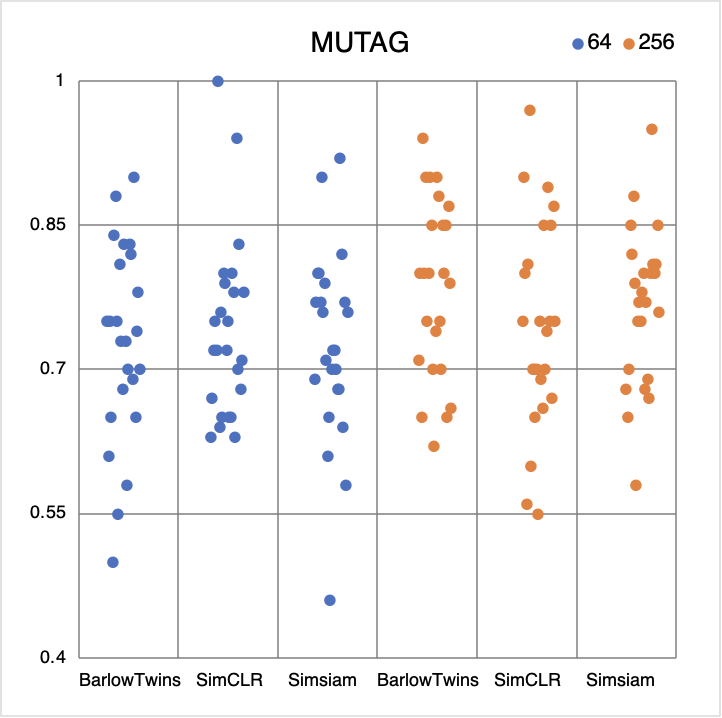
\includegraphics[width = .48\linewidth]{./figures/3-MUTAG.png}\quad
        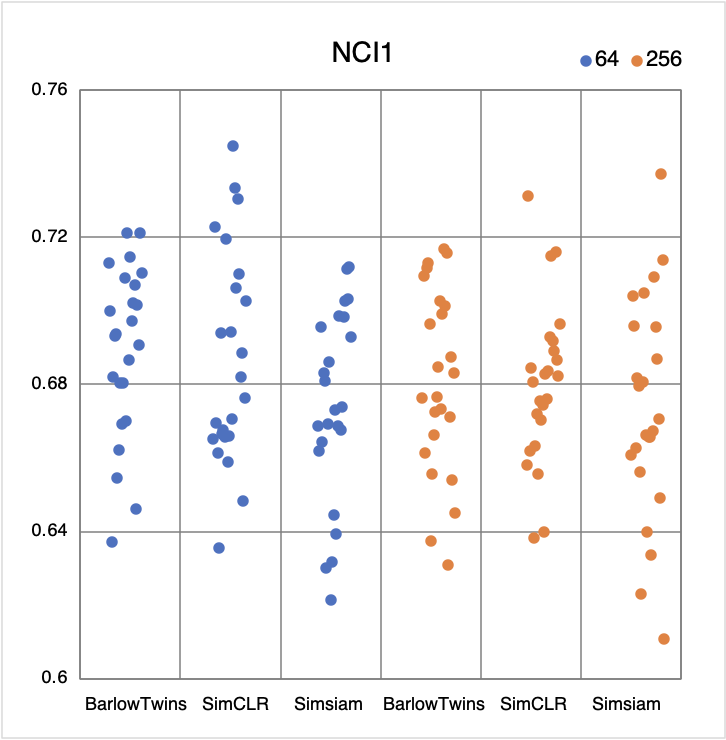
\includegraphics[width = .48\linewidth]{./figures/3-NCI1.png}}
\subcaptionbox{Bioinformatics Dataset\label{subfig:simclrbatch_bio}}
    {%
        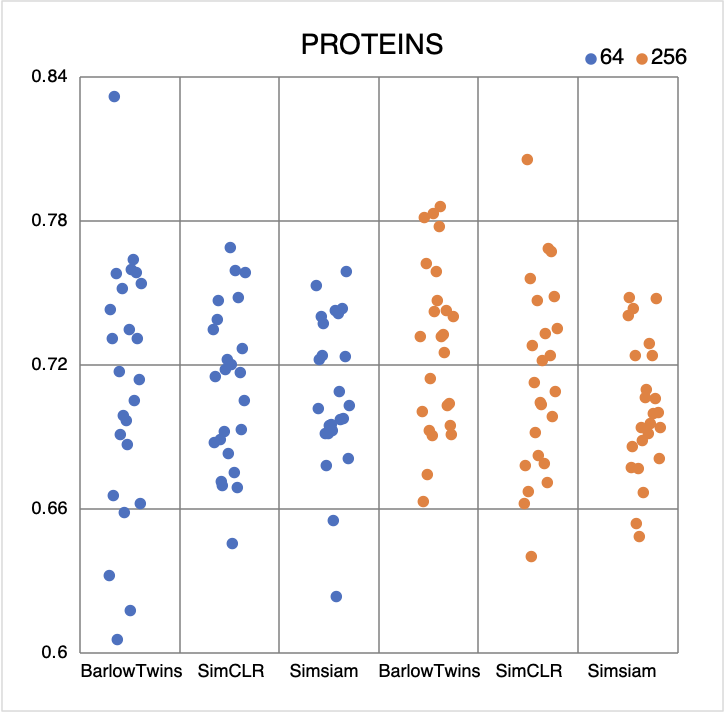
\includegraphics[width = .48\linewidth]{./figures/3-PROTEINS.png}\quad
        % \subcaptionbox{below\label{subfig:below}}
        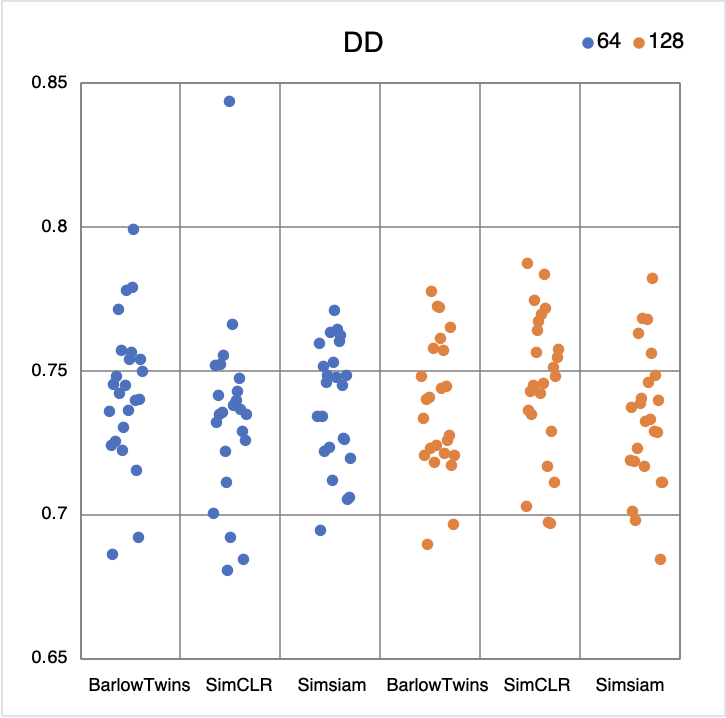
\includegraphics[width = .48\linewidth]{./figures/3-DD.png}}
\vspace{0.5cm}
\caption[Evaluation using different batch sizes]{\textbf{Evaluation using different batch sizes.} In this figure, each colored dot represents the average accuracy of experiment after five times repetitions. By grouping experiments that use the same batch sizes, we use blue and orange colors to indicate the effect of different batch sizes in different types of models. For example, in the leftmost column of each figure, the blue dots represent the performance of a model that uses Barlow Twins and 64 mini-batches.} \label{fig:simclrbatch}
\end{figure}




%%%%%%%%%%%%%%%%%%%%%%%%%%%%%%%%%%%%%%%%%%%%%%%%%%%%%%%%%%%%%%%%
%%%%%%%%%%%%%%%%%%%%%%%%%%%%%%%%%%%%%%%%%%%%%%%%%%%%%%%%%%%%%%%%
%%%%%%%%%%%%%%%%%%%%%%%%%%%%%%%%%%%%%%%%%%%%%%%%%%%%%%%%%%%%%%%%




\section{Deeper encoders have better performance}

Generally, models using a deep encoder are thought to have better performance than others using a shallow encoder. To judge this idea on graph datasets, we have tested three types of encoders, namely, monolayer, bilayer, and trilayer, during the training stage. 

For an encoder with a monolayer, the MLP part consists of a linear layer, followed by a ReLU layer and another linear layer. We used a graph isomorphism network encoder to generate embeddings of samples. For bilayer and trilayer architectures, the MLP parts consist of several monolayers stacked and connected by batch normalization layers.

Figure \ref{fig:deeper} shows that the medians and quartiles of accuracy are higher for models with deeper encoders. Such superior performance is particularly obvious when models are trained on the MUTAG, NCI1, and PROTEINS datasets.

Following the experiment results, the hypothesis that the deeper encoder also benefits from the graph-structured model is verified through the analysis. Future self-supervised methods should concentrate on the deeper architecture.


\begin{figure}[htbp]
\centering
\subcaptionbox{Molecular Dataset\label{subfig:deeper_mol}}
    {%
        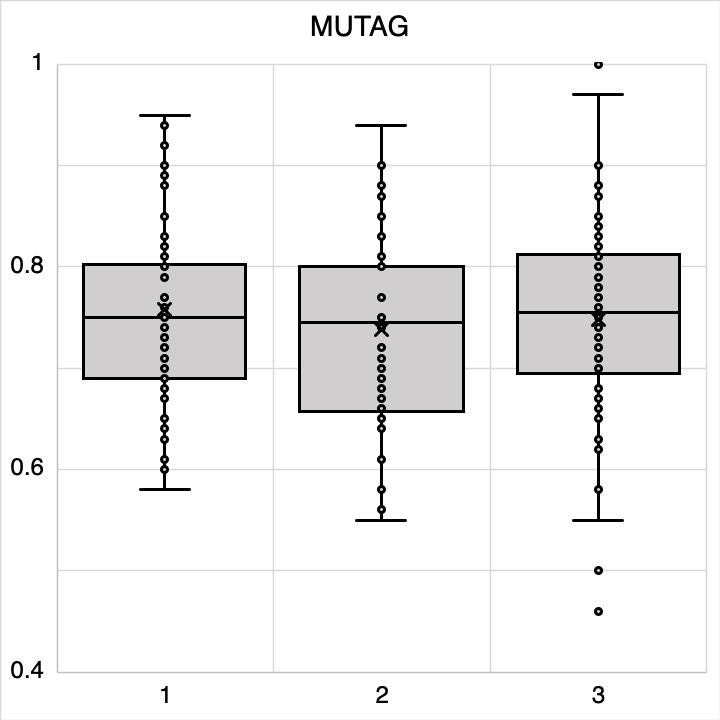
\includegraphics[width = .48\linewidth]{./figures/4-MUTAG.png}\quad
        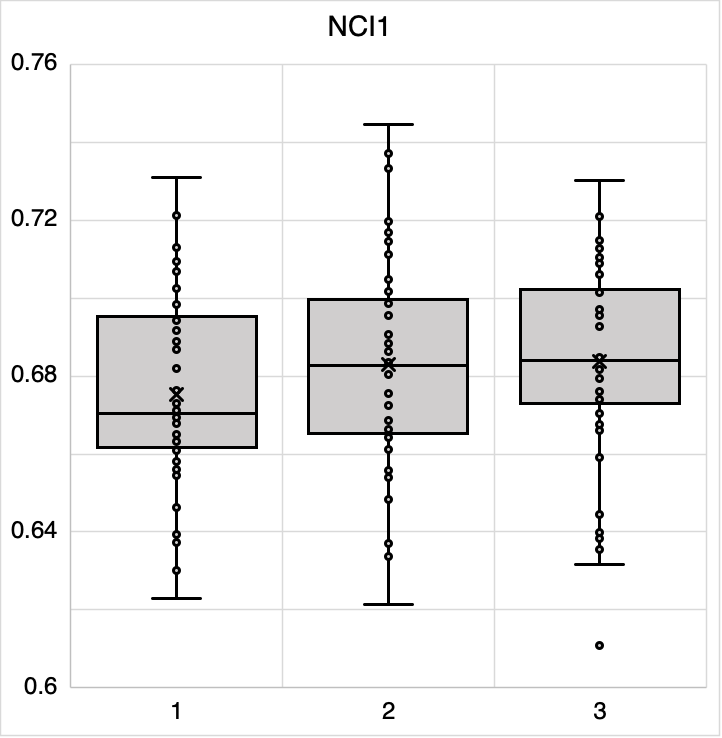
\includegraphics[width = .48\linewidth]{./figures/4-NCI1.png}}
\subcaptionbox{Bioinformatics Dataset\label{subfig:deeper_bio}}
    {%
        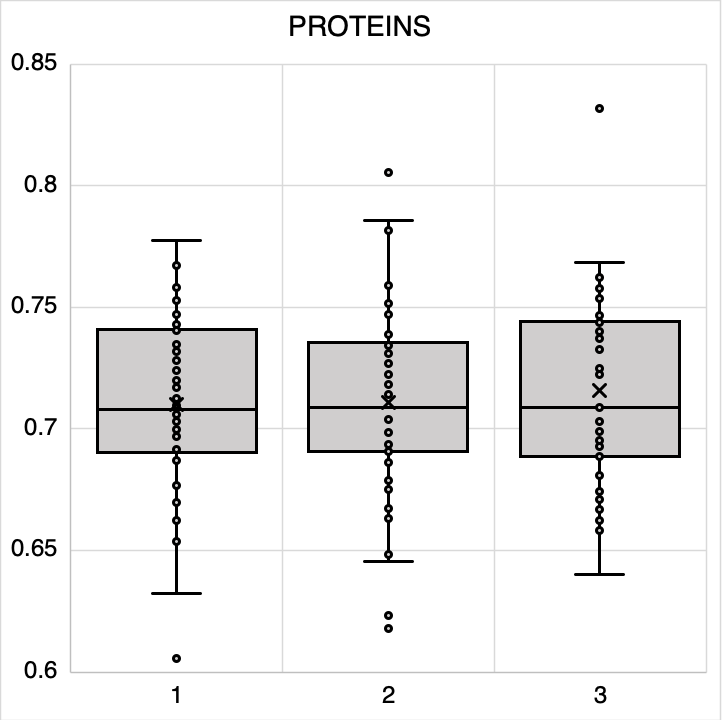
\includegraphics[width = .48\linewidth]{./figures/4-PROTEINS.png}\quad
        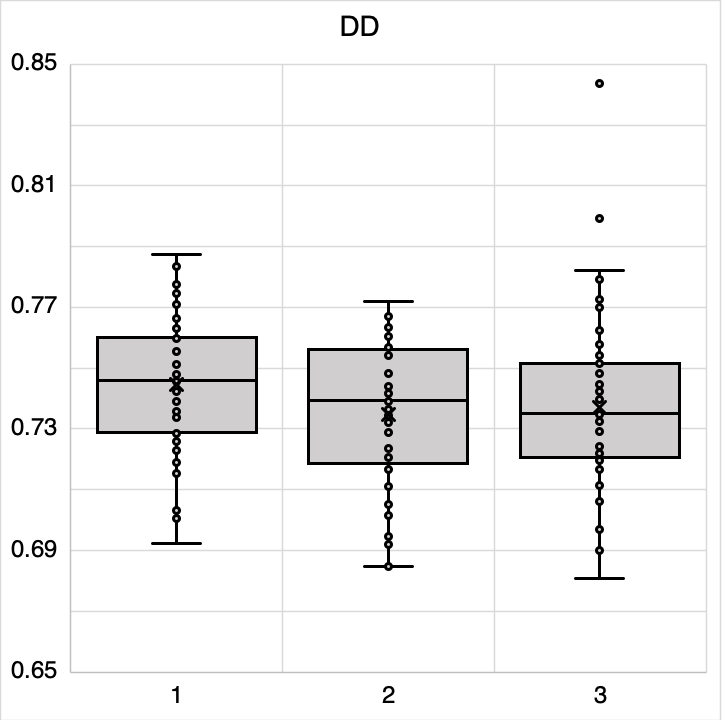
\includegraphics[width = .48\linewidth]{./figures/4-DD.png}}
\vspace{0.5cm}
\caption[Evaluation using different depths of an encoder layer]{\textbf{Evaluation using different depths of an encoder layer.} In this figure, each gray dot represents the average accuracy of experiment after five times repetitions. By grouping experiments that use the same depths of the encoder layer, we can observe the minimum, median, maximum, and quartile performance under different encoder depths. For example, in the leftmost column of each figure, the gray nodes represent the performance of a model that uses used a monolayer encoder.}\label{fig:deeper}
\end{figure}


%%%%%%%%%%%%%%%%%%%%%%%%%%%%%%%%%%%%%%%%%%%%%%%%%%%%%%%%%%%%%%%%
%%%%%%%%%%%%%%%%%%%%%%%%%%%%%%%%%%%%%%%%%%%%%%%%%%%%%%%%%%%%%%%%
%%%%%%%%%%%%%%%%%%%%%%%%%%%%%%%%%%%%%%%%%%%%%%%%%%%%%%%%%%%%%%%%


\section{Hidden dimension has little effect on model performance}

In most state-of-the-art neural networks, especially in image processing, NLP, and classification tasks, the hidden dimension of each encoder layer influences model performance. The hidden dimension determines the size of the feature vector. As the hidden dimension increases, an encoder can capture more complex features as hidden states, resulting in a more comprehensive representation of data.

However, in our experiment, we tested 64 and 512 hidden dimensions for models trained on the MUTAG, NCI1, and PROTEINS and tested 64 and 128 for models trained on the DD dataset. Figure \ref{fig:hidden} shows that accuracy varies across different hidden dimensions. For models with 512 hidden dimensions, even if the vector size is eight times larger than those with 64 hidden dimensions, there is no significant improvement in model performance. 

These surprising differences can be explained in part by the data structure of graph and image data. For image data, which consist of discrete pixels, with a larger hidden dimension, a neuron can capture more information via pixel clustering. However, graph data are more abstract. Nodes and edges cannot be separated or unified as pixel groups in image data. This difference makes adding hidden dimensions less effective in model training. 

In summary, if we want to apply a self-supervised method to graph data, increasing the hidden dimension size may not be helpful. However, if the raw data can be discretization into small units, such as an image into pixels, or a sentence into n-gram, increasing the hidden dimension size is a reliable way to improve performance. 


\begin{figure}[htbp]
\centering
\subcaptionbox{Molecular Dataset\label{subfig:hidden_mol}}
    {%
        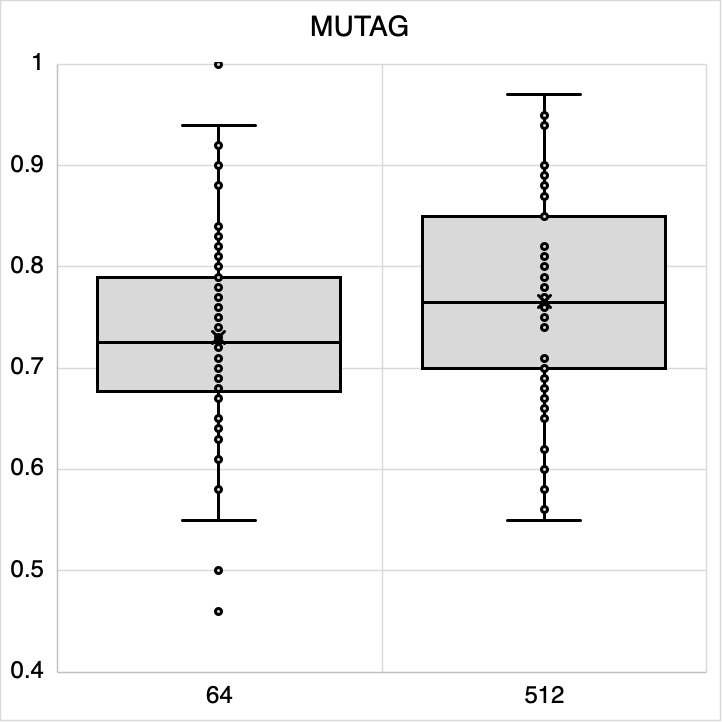
\includegraphics[width = .48\linewidth]{./figures/5-MUTAG.png}\quad
        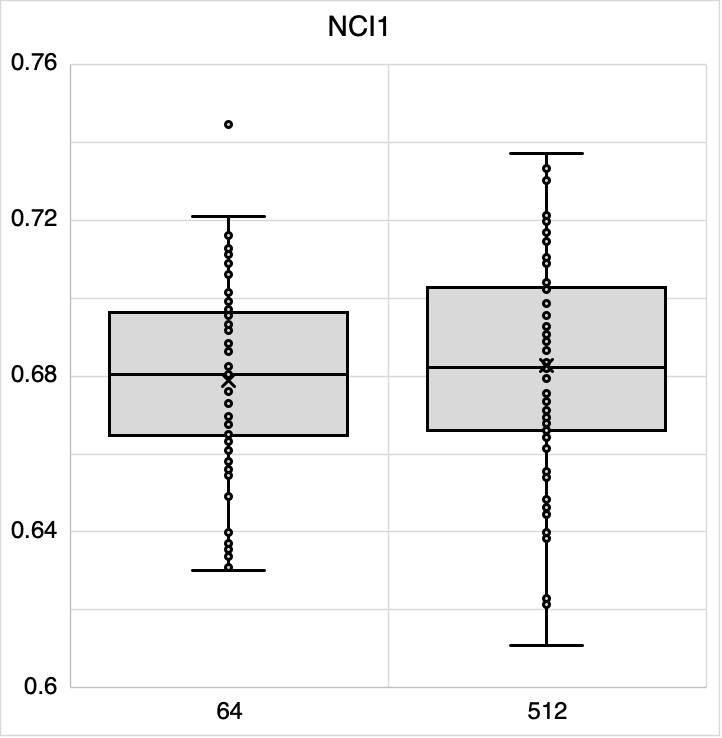
\includegraphics[width = .48\linewidth]{./figures/5-NCI1.png}}
\subcaptionbox{Bioinformatics Dataset\label{subfig:hidden_bio}}
    {%
        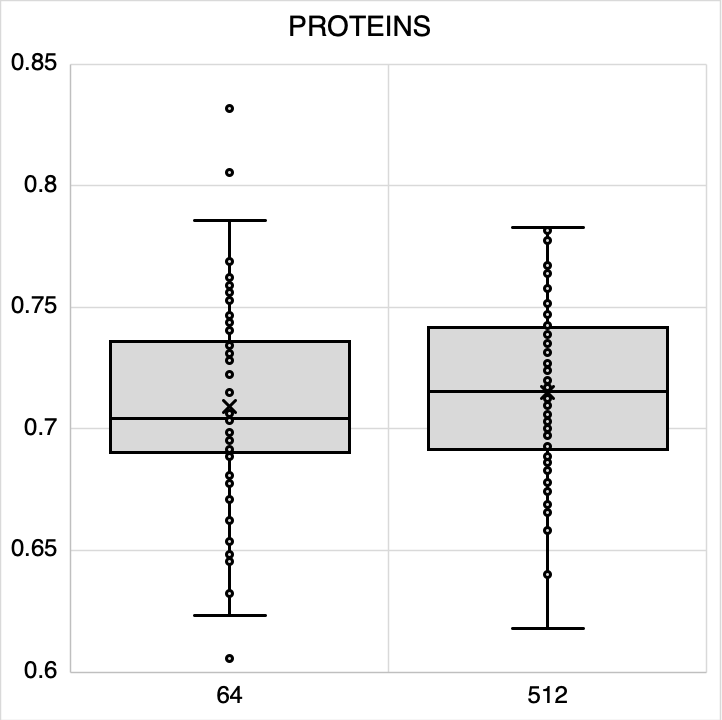
\includegraphics[width = .48\linewidth]{./figures/5-PROTEINS.png}\quad
        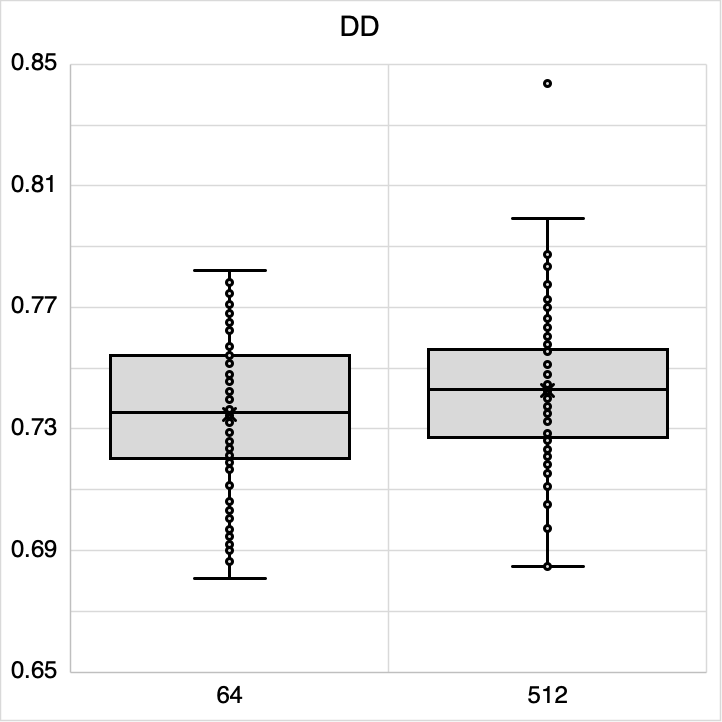
\includegraphics[width = .48\linewidth]{./figures/5-DD.png}}
\vspace{0.5cm}
\caption[Evaluation using different hidden dimensions]{\textbf{Evaluation using different hidden dimensions.} In this figure, each gray dot represents the average accuracy of experiment after five times repetitions. By grouping experiments that use the same hidden dimensions, we can observe the minimum, median, maximum, and quartile performance under different hidden dimensions in the hidden layer. For example, in the leftmost column of each figure, the gray dots represent the performance of a model that uses 64 hidden dimensions.}\label{fig:hidden}
\end{figure}


%%%%%%%%%%%%%%%%%%%%%%%%%%%%%%%%%%%%%%%%%%%%%%%%%%%%%%%%%%%%%%%%
%%%%%%%%%%%%%%%%%%%%%%%%%%%%%%%%%%%%%%%%%%%%%%%%%%%%%%%%%%%%%%%%
%%%%%%%%%%%%%%%%%%%%%%%%%%%%%%%%%%%%%%%%%%%%%%%%%%%%%%%%%%%%%%%%


\section{SimCLR performs better in molecular datasets}

In our experiments, we used four datasets, of which two, MUTAG and NCI1, are molecular datasets. The other two datasets, PROTEINS and DD, are bioinformatics datasets. Figure \ref{fig:simclrbetter} shows that models trained via SimCLR performed better than models trained via the other approaches on both molecular datasets. Conversely, models trained via SimCLR did not outperform models trained via Barlow Twins and Simsiam on bioinformatics datasets.

Reviewing these datasets will help us understand why performance varies. Although these data are graph-structured, there are fundamental differences between molecular and bioinformatics graph data. In molecular datasets, e.g., MUTAG and NCI1, each node represents an atom, and each edge represents a chemical bond connecting two nodes. In bioinformatics datasets, such as PROTEINS and DD, each node represents an amino acid, and two nodes are connected by an edge if they are less than 6 angstroms apart.

Both types of datasets have different types of properties, which can have complex effects on self-supervised models. Unlike Simsiam that only uses one projection, or Barlow Twins that uses embeddings directly, in the SimCLR architecture, raw data and augmented data are encoded into projections, which may affect performance.

The experimental results indicate that SimCLR is a suitable application model for molecular datasets; however, more empirical experiments are required to verify its robustness. Unfortunately, at present, owing to computational power constraints, this study lacks experimental logs of larger molecular datasets. A further study focusing on SimCLR or molecular graph-structured datasets should be conducted.


\begin{figure}
\centering
\subcaptionbox{Molecular Dataset\label{subfig:simclrbetter_mol}}
    {%
        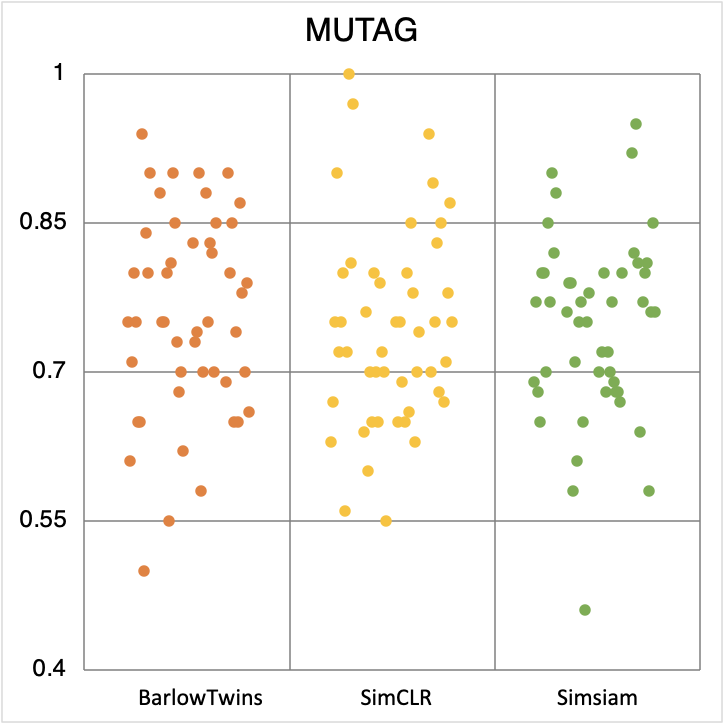
\includegraphics[width = .48\linewidth]{./figures/1-MUTAG.png}\quad
        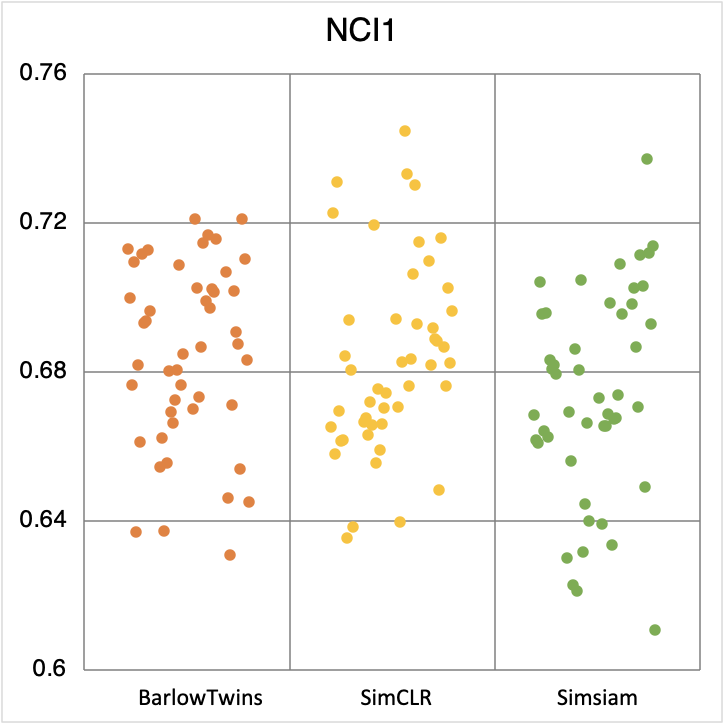
\includegraphics[width = .48\linewidth]{./figures/1-NCI1.png}}
\subcaptionbox{Bioinformatics Dataset\label{subfig:simclrbetter_bio}}
    {%
        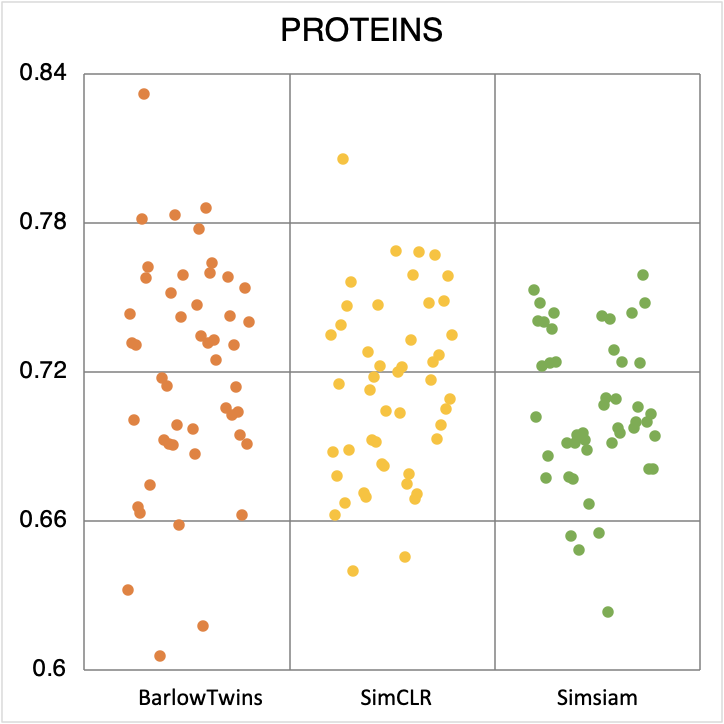
\includegraphics[width = .48\linewidth]{./figures/1-PROTEINS.png}\quad
        % \subcaptionbox{below\label{subfig:below}}
        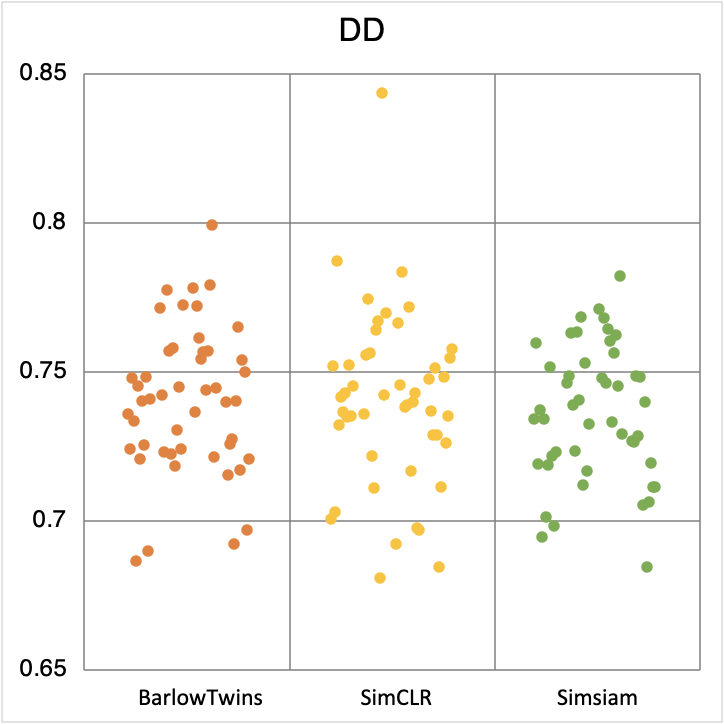
\includegraphics[width = .48\linewidth]{./figures/1-DD.png}}
\vspace{0.5cm}
\caption[Evaluation using different self-supervised methods]{\textbf{Evaluation using different self-supervised methods.} In this figure, each colored dot represents the average accuracy of experiment. By grouping experiments that use the same approaches, we use orange, yellow, and green colors to indicate the evaluation via Barlow Twins, SimCLR, and Simsiam, respectively. For example, in the leftmost column of each figure, the orange dots represent the performance of a model that uses Barlow Twins.}
\label{fig:simclrbetter}
\end{figure}


%%%%%%%%%%%%%%%%%%%%%%%%%%%%%%%%%%%%%%%%%%%%%%%%%%%%%%%%%%%%%%%%
%%%%%%%%%%%%%%%%%%%%%%%%%%%%%%%%%%%%%%%%%%%%%%%%%%%%%%%%%%%%%%%%
%%%%%%%%%%%%%%%%%%%%%%%%%%%%%%%%%%%%%%%%%%%%%%%%%%%%%%%%%%%%%%%%

\section{SUBGRAPH augmentation performs closer in bioinformatics dataset}

Furthermore, there is an interesting discovery in our experiment results. The idea behind data augmentation, especially in the SUBGRAPH operator, assumes that the partial graph should retain the properties of the entire graph, even when some nodes or edges are added or removed.  

From Figure \ref{fig:stable} shows that models trained using the SUBGRAPH operator achieve similar performance on the DD and PROTEINS datasets. The variance in performance was lower than those on the molecular datasets.

As previously mentioned, molecular and bioinformatics datasets have different properties and targets. First, the goal of MUTAG is to train models to predict the mutagenicity of Salmonella typhimurium. Second, the goal of NCI1 is to train models to classify whether a chemical compound is positive or negative for cell lung cancer. Third, the goal of the PROTEINS and DD datasets is to train models to predict which proteins are enzymes or non-enzymes.

In a chemical molecule, each node and edge play a unique role. The functional group may be lost if we only capture a part of the graph. For example, the chemical formula of ethanol (a.k.a. alcohol) is $\text{C}_{2}\text{H}_{5}\text{OH}$, containing a hydroxyl group (-OH). If the augmented operator samples $\text{C}_{2}\text{H}_{4}$, it will be recognized as ethene, which has different chemical properties from ethanol. Because the augmented data have more diversity, the performance of the model will have a higher variance.

In contrast, a protein contains at least one long polypeptide, which is chained by amino acid. Proteins can be constructed in flexible ways \cite{accurateprotein}. Some proteins chained by different polypeptides can have similar chemical properties and functions. Therefore, even when we use the SUBGRAPH operator, the augmented data are similar to the raw data, reducing the variance between experiment results.

This finding, while preliminary, suggests that augmented data generated using the SUBGRAPH operator should be carefully used. To avoid a good experiment result producing trivial analysis, we should first observe the representation of each node and edge and consider their chemical and physic attributes before attempting to sample raw data as augmentation data.

\begin{figure}
\centering
\subcaptionbox{Molecular Dataset\label{subfig:stable_mol}}
    {%
        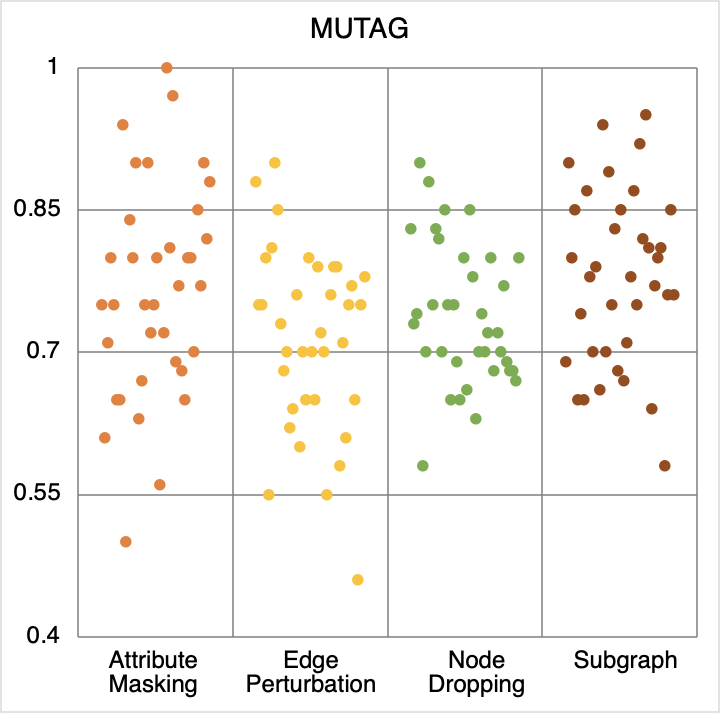
\includegraphics[width = .48\linewidth]{./figures/2-MUTAG.png}\quad
        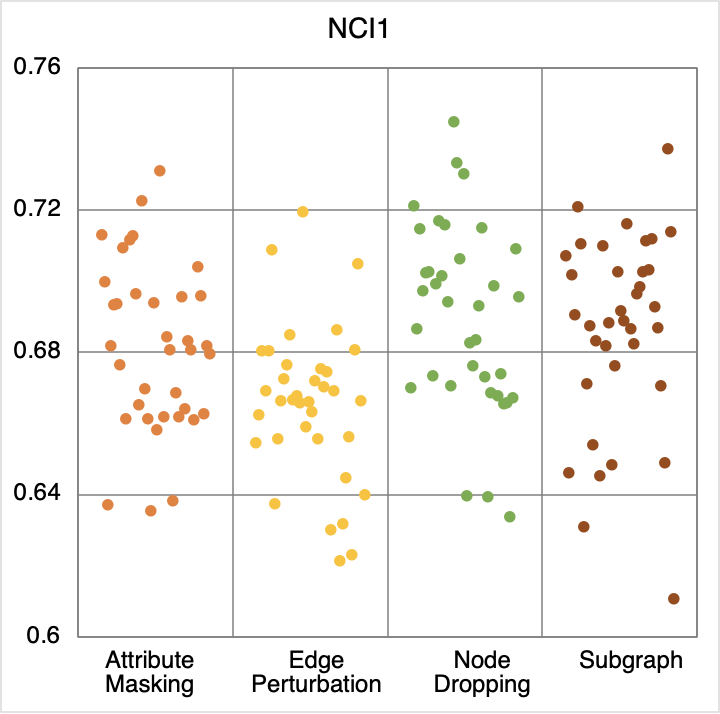
\includegraphics[width = .48\linewidth]{./figures/2-NCI1.png}}
\subcaptionbox{Bioinformatics Dataset\label{subfig:stable_bio}}
    {%
        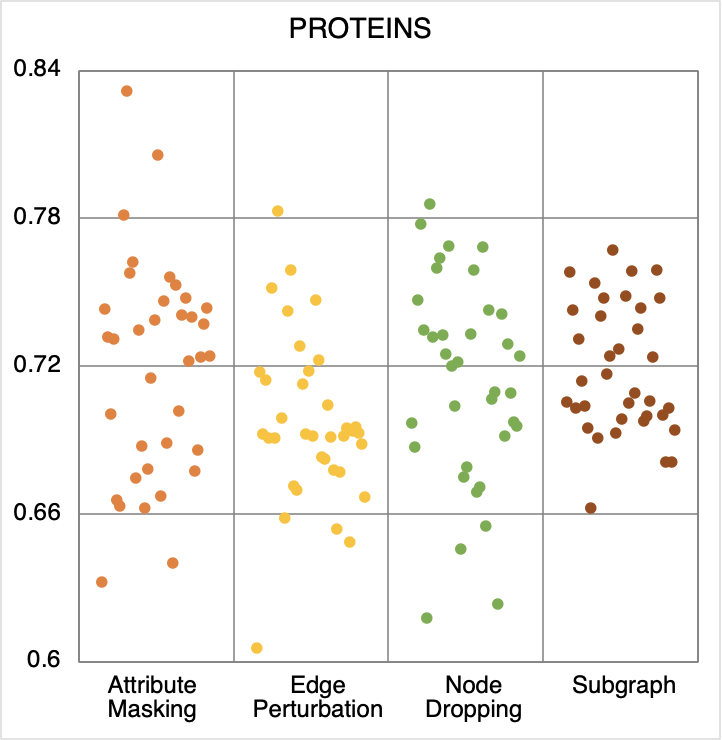
\includegraphics[width = .48\linewidth]{./figures/2-PROTEINS.png}\quad
        % \subcaptionbox{below\label{subfig:below}}
        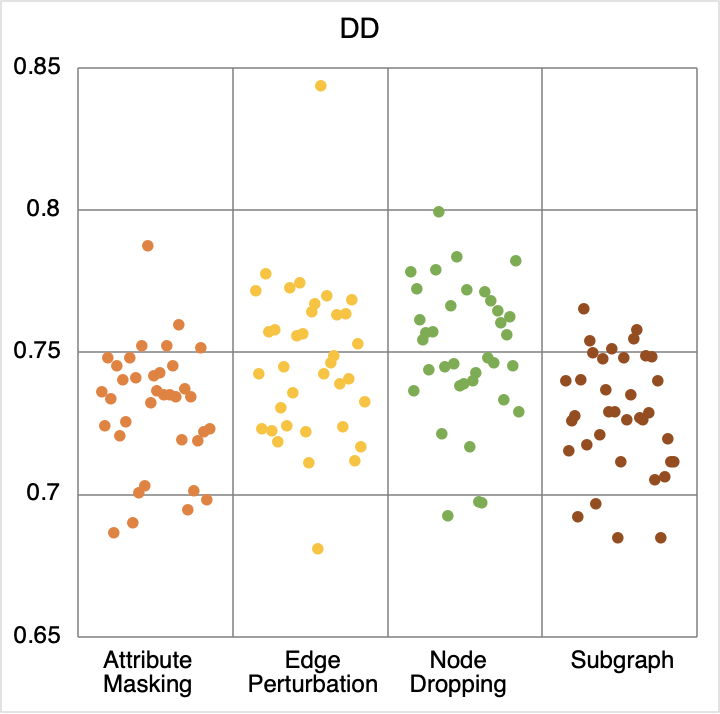
\includegraphics[width = .48\linewidth]{./figures/2-DD.png}}
\vspace{0.5cm}
\caption[SUBGRAPH augmentation performs better on bioinformatics datasets]{\textbf{SUBGRAPH augmentation performs better on bioinformatics datasets.} In this figure, each colored dot represents the average accuracy of experiment. By grouping experiments that use the same data augmentation method, we use orange, yellow, green, and brown colors to indicate the evaluation by ATTRIBUTE MASKING, EDGE PERTUBATION, NODE DROPPING, and SUBGRAPH, respectively. For example, in the leftmost column of each figure, the orange dots represent the performance of a model that uses ATTRIBUTE MASKING to generate augmented data.}
\label{fig:stable}
\end{figure}


%%%%%%%%%%%%%%%%%%%%%%%%%%%%%%%%%%%%%%%%%%%%%%%%%%%%%%%%%%%%%%%%
%%%%%%%%%%%%%%%%%%%%%%%%%%%%%%%%%%%%%%%%%%%%%%%%%%%%%%%%%%%%%%%%
%%%%%%%%%%%%%%%%%%%%%%%%%%%%%%%%%%%%%%%%%%%%%%%%%%%%%%%%%%%%%%%%


\section{Discussion}

Most studies on self-supervised learning have only been conducted in image processing and NLP. In this chapter, we have revised the properties of graph data, analyzed the experimental results, and attempted to provide some possible explanations. 

According to our findings, not all hyperparameters influence model performance significantly. Some of them only have a small effect when the dataset size is not sufficiently large. On the other hand, the fundamental differences between graphs and other data structures, along with the categories of graph datasets, prevent models from applying the same training strategies.
% !TeX root = ../main.tex

\section{Conclusion}\label{sec:5}

We have systematically investigated three self-supervised learning methods by employing them to train DNNs on graph data. We have also discussed the simulation experiments in detail, providing explanations for the experiment results so that subsequent researchers may use them to propose better methods and ideas.

First, increasing the batch size in the training stage when the dataset is medium or small size is not helpful, but deepening the layer of the encoder seems to be a favorable means to improve model performance. Second, graphs have their special structure. Applying previous procedures used to improve the performance of models trained on image datasets, e.g., increasing the hidden dimension size, to every similar scenario may not be inappropriate. Finally, because of the characteristic differences between molecular and bioinformatics data, different optimal hyperparameters should be used when training models on these two data types.

At present, we only focus on small-scale datasets containing less than ten thousand samples. However, real-world data generated by commercial systems may have millions of nodes or 10 billion edges, which are orders of magnitude larger than the datasets used in this thesis. Owing to resource constraints and computational limitations, we cannot provide a comprehensive review of larger graph datasets. 


There is abundant space for advancement in large-scale datasets \cite{choi2022triangular} and other categories, such as social networks or recommendation systems \cite{mahcl}. Furthermore, future research should explore new data augmentation methods \cite{yang2022contrastive, shen2022improving}, as well as other key factors in or approaches \cite{hou2022graphmae} to self-supervised learning, to find a robust and efficient method for improving model performance.





% 參考文獻
% References
\refmatter
\bibliographystyle{abbrv}
\bibliography{back/references}

% 附錄
% Appendices
% !TeX root = ../main.tex

\section{Appendix: Experiment Result}

In the Table mentioned below, red colored values represent the best models in the training and test stages.

The source code and full experiment logs aref available on Github:

https://github.com/rutopio/Training-Graph-Neural-Networks-via-Self-Supervised-Learning


\subsection{Performance on MUTAG dataset}

Table \ref{tab:mutag} shows the experiment results of models trained on MUTAG dataset. Noticed that MUTAG is a relatively small dataset, which only has 188 graphs, so 100\% accuracy is possible. 

The best setting in the training stage is the one that uses SimCLR with Attribute Masking, batch size set to 64 hidden dimension set to 512, and using a trilayer MLP as the encoder.

The best setting in the test stage is the one that uses SimCLR with Attribute Masking, batch size set to 64, hidden dimension set to 512, and using a trilayer MLP as the encoder.




\begin{table}[htpb]
\centering
\resizebox{1\textwidth}{!}{
\begin{tabular}{c|c|c|c|rr|rr|rr|rr}
\hline
                                 &                                                                                 &                                                                                        &                                                                                           & \multicolumn{2}{c|}{\textbf{Node Droppping}}                                      & \multicolumn{2}{c|}{\textbf{Edge Pertubation}}                                    & \multicolumn{2}{c|}{\textbf{Attribute Masking}}                                     & \multicolumn{2}{c}{\textbf{Subgraph}}                                            \\ \cline{5-12} 
\multirow{-2}{*}{\textbf{Model}} & \multirow{-2}{*}{\textbf{\begin{tabular}[c]{@{}c@{}}Batch\\ Size\end{tabular}}} & \multirow{-2}{*}{\textbf{\begin{tabular}[c]{@{}c@{}}Hidden \\ Dimension\end{tabular}}} & \multirow{-2}{*}{\textbf{\begin{tabular}[c]{@{}c@{}}\# Layer \\ of Encoder\end{tabular}}} & \multicolumn{1}{c}{\textbf{Train Acc.}} & \multicolumn{1}{c|}{\textbf{Test Acc.}} & \multicolumn{1}{c}{\textbf{Train Acc.}} & \multicolumn{1}{c|}{\textbf{Test Acc.}} & \multicolumn{1}{c}{\textbf{Train Acc.}}  & \multicolumn{1}{c|}{\textbf{Test Acc.}}  & \multicolumn{1}{c}{\textbf{Train Acc.}} & \multicolumn{1}{c}{\textbf{Test Acc.}} \\ \hline
                                 &                                                                                 &                                                                                        & 1                                                                                         & 72.000$\pm$2.739                        & 75.000$\pm$6.124                        & 76.000$\pm$2.236                        & 64.000$\pm$5.477                        & 75.000$\pm$0.000                         & 63.000$\pm$4.472                         & 79.000$\pm$2.236                        & 94.000$\pm$2.236                       \\
                                 &                                                                                 &                                                                                        & 2                                                                                         & 75.000$\pm$0.000                        & 65.000$\pm$0.000                        & 65.000$\pm$0.000                        & 65.000$\pm$0.000                        & 78.000$\pm$4.472                         & 72.000$\pm$4.472                         & 84.000$\pm$2.236                        & 83.000$\pm$4.472                       \\
                                 &                                                                                 & \multirow{-3}{*}{64}                                                                   & 3                                                                                         & 74.000$\pm$7.416                        & 78.000$\pm$7.583                        & 84.000$\pm$5.477                        & 79.000$\pm$6.519                        & 87.000$\pm$2.739                         & 72.000$\pm$2.739                         & 77.000$\pm$2.739                        & 71.000$\pm$2.236                       \\ \cline{3-12} 
                                 &                                                                                 &                                                                                        & 1                                                                                         & 80.000$\pm$0.000                        & 65.000$\pm$0.000                        & 78.000$\pm$6.708                        & 76.000$\pm$2.236                        & 75.000$\pm$0.000                         & 67.000$\pm$2.739                         & 85.000$\pm$0.000                        & 70.000$\pm$0.000                       \\
                                 &                                                                                 &                                                                                        & 2                                                                                         & 81.000$\pm$4.183                        & 80.000$\pm$0.000                        & 78.000$\pm$2.739                        & 80.000$\pm$0.000                        & 85.000$\pm$0.000                         & 75.000$\pm$0.000                         & 88.000$\pm$2.739                        & 68.000$\pm$5.701                       \\
                                 & \multirow{-6}{*}{64}                                                            & \multirow{-3}{*}{512}                                                                  & 3                                                                                         & 77.000$\pm$2.739                        & 63.000$\pm$4.472                        & 80.000$\pm$0.000                        & 72.000$\pm$2.739                        & {\color[HTML]{FE0000} 100.000$\pm$0.000} & {\color[HTML]{FE0000} 100.000$\pm$0.000} & 85.000$\pm$0.000                        & 78.000$\pm$5.701                       \\ \cline{2-12} 
                                 &                                                                                 &                                                                                        & 1                                                                                         & 75.000$\pm$0.000                        & 75.000$\pm$0.000                        & 75.000$\pm$0.000                        & 60.000$\pm$0.000                        & 69.000$\pm$5.477                         & 75.000$\pm$0.000                         & 78.000$\pm$4.472                        & 89.000$\pm$2.236                       \\
                                 &                                                                                 &                                                                                        & 2                                                                                         & 76.000$\pm$2.236                        & 66.000$\pm$2.236                        & 71.000$\pm$2.236                        & 70.000$\pm$0.000                        & 81.000$\pm$4.183                         & 80.000$\pm$0.000                         & 76.000$\pm$2.236                        & 85.000$\pm$0.000                       \\
                                 &                                                                                 & \multirow{-3}{*}{64}                                                                   & 3                                                                                         & 73.000$\pm$2.739                        & 70.000$\pm$0.000                        & 75.000$\pm$0.000                        & 70.000$\pm$0.000                        & 89.000$\pm$4.183                         & 81.000$\pm$8.216                         & 78.000$\pm$6.708                        & 87.000$\pm$2.739                       \\ \cline{3-12} 
                                 &                                                                                 &                                                                                        & 1                                                                                         & 80.000$\pm$0.000                        & 69.000$\pm$2.236                        & 65.000$\pm$0.000                        & 70.000$\pm$0.000                        & 77.000$\pm$2.739                         & 90.000$\pm$0.000                         & 85.000$\pm$0.000                        & 75.000$\pm$0.000                       \\
                                 &                                                                                 &                                                                                        & 2                                                                                         & 71.000$\pm$2.236                        & 85.000$\pm$0.000                        & 72.000$\pm$2.739                        & 65.000$\pm$0.000                        & 82.000$\pm$2.739                         & 56.000$\pm$2.236                         & 85.000$\pm$0.000                        & 67.000$\pm$5.701                       \\
\multirow{-12}{*}{SimCLR}        & \multirow{-6}{*}{256}                                                           & \multirow{-3}{*}{512}                                                                  & 3                                                                                         & 76.000$\pm$2.236                        & 74.000$\pm$2.236                        & 75.000$\pm$0.000                        & 55.000$\pm$0.000                        & 99.000$\pm$2.236                         & 97.000$\pm$6.708                         & 85.000$\pm$0.000                        & 75.000$\pm$0.000                       \\ \hline
                                 &                                                                                 &                                                                                        & 1                                                                                         & 80.000$\pm$0.000                        & 70.000$\pm$0.000                        & 76.000$\pm$2.236                        & 76.000$\pm$2.236                        & 74.000$\pm$5.477                         & 69.000$\pm$4.183                         & 83.000$\pm$2.739                        & 92.000$\pm$2.739                       \\
                                 &                                                                                 &                                                                                        & 2                                                                                         & 75.000$\pm$0.000                        & 72.000$\pm$2.739                        & 73.000$\pm$2.739                        & 71.000$\pm$4.183                        & 81.000$\pm$4.183                         & 80.000$\pm$5.000                         & 78.000$\pm$4.472                        & 64.000$\pm$6.519                       \\
                                 &                                                                                 & \multirow{-3}{*}{64}                                                                   & 3                                                                                         & 80.000$\pm$3.536                        & 68.000$\pm$2.739                        & 79.000$\pm$5.477                        & 65.000$\pm$0.000                        & 84.000$\pm$4.183                         & 77.000$\pm$2.739                         & 72.000$\pm$6.708                        & 58.000$\pm$4.472                       \\ \cline{3-12} 
                                 &                                                                                 &                                                                                        & 1                                                                                         & 82.000$\pm$2.739                        & 72.000$\pm$2.739                        & 76.000$\pm$2.236                        & 79.000$\pm$2.236                        & 80.000$\pm$5.000                         & 77.000$\pm$4.472                         & 87.000$\pm$4.472                        & 82.000$\pm$4.472                       \\
                                 &                                                                                 &                                                                                        & 2                                                                                         & 75.000$\pm$0.000                        & 70.000$\pm$0.000                        & 76.000$\pm$2.236                        & 61.000$\pm$2.236                        & 83.000$\pm$2.739                         & 80.000$\pm$3.536                         & 78.000$\pm$4.472                        & 77.000$\pm$7.583                       \\
                                 & \multirow{-6}{*}{64}                                                            & \multirow{-3}{*}{512}                                                                  & 3                                                                                         & 73.000$\pm$2.739                        & 68.000$\pm$2.739                        & 80.000$\pm$0.000                        & 46.000$\pm$5.477                        & 90.000$\pm$3.536                         & 90.000$\pm$5.000                         & 80.000$\pm$11.726                       & 76.000$\pm$6.519                       \\ \cline{2-12} 
                                 &                                                                                 &                                                                                        & 1                                                                                         & 74.000$\pm$4.183                        & 80.000$\pm$0.000                        & 72.000$\pm$4.472                        & 79.000$\pm$2.236                        & 75.000$\pm$0.000                         & 68.000$\pm$4.472                         & 79.000$\pm$5.477                        & 95.000$\pm$0.000                       \\
                                 &                                                                                 &                                                                                        & 2                                                                                         & 76.000$\pm$2.236                        & 77.000$\pm$2.739                        & 77.000$\pm$6.708                        & 75.000$\pm$0.000                        & 72.000$\pm$4.472                         & 70.000$\pm$0.000                         & 80.000$\pm$3.536                        & 80.000$\pm$0.000                       \\
                                 &                                                                                 & \multirow{-3}{*}{64}                                                                   & 3                                                                                         & 74.000$\pm$2.236                        & 67.000$\pm$2.739                        & 75.000$\pm$0.000                        & 75.000$\pm$0.000                        & 82.000$\pm$2.739                         & 82.000$\pm$2.739                         & 81.000$\pm$2.236                        & 85.000$\pm$0.000                       \\ \cline{3-12} 
                                 &                                                                                 &                                                                                        & 1                                                                                         & 83.000$\pm$2.739                        & 68.000$\pm$2.739                        & 77.000$\pm$2.739                        & 58.000$\pm$5.701                        & 79.000$\pm$2.236                         & 65.000$\pm$0.000                         & 84.000$\pm$2.236                        & 81.000$\pm$5.477                       \\
                                 &                                                                                 &                                                                                        & 2                                                                                         & 79.000$\pm$6.519                        & 69.000$\pm$9.618                        & 77.000$\pm$4.472                        & 77.000$\pm$4.472                        & 78.000$\pm$5.701                         & 85.000$\pm$0.000                         & 81.000$\pm$6.519                        & 81.000$\pm$2.236                       \\
\multirow{-12}{*}{Simsiam}       & \multirow{-6}{*}{256}                                                           & \multirow{-3}{*}{512}                                                                  & 3                                                                                         & 72.000$\pm$10.368                       & 80.000$\pm$0.000                        & 76.000$\pm$4.183                        & 78.000$\pm$2.739                        & 82.000$\pm$4.472                         & 88.000$\pm$10.954                        & 77.000$\pm$8.367                        & 76.000$\pm$5.477                       \\ \hline
                                 &                                                                                 &                                                                                        & 1                                                                                         & 75.000$\pm$0.000                        & 83.000$\pm$4.472                        & 75.000$\pm$0.000                        & 88.000$\pm$2.739                        & 75.000$\pm$0.000                         & 75.000$\pm$0.000                         & 83.000$\pm$2.739                        & 69.000$\pm$2.236                       \\
                                 &                                                                                 &                                                                                        & 2                                                                                         & 80.000$\pm$0.000                        & 58.000$\pm$2.739                        & 73.000$\pm$4.472                        & 55.000$\pm$0.000                        & 80.000$\pm$3.536                         & 75.000$\pm$0.000                         & 80.000$\pm$5.000                        & 65.000$\pm$0.000                       \\
                                 &                                                                                 & \multirow{-3}{*}{64}                                                                   & 3                                                                                         & 76.000$\pm$2.236                        & 83.000$\pm$4.472                        & 75.000$\pm$0.000                        & 73.000$\pm$2.739                        & 74.000$\pm$4.183                         & 50.000$\pm$6.124                         & 82.000$\pm$4.472                        & 78.000$\pm$5.701                       \\ \cline{3-12} 
                                 &                                                                                 &                                                                                        & 1                                                                                         & 80.000$\pm$0.000                        & 73.000$\pm$2.739                        & 85.000$\pm$0.000                        & 75.000$\pm$0.000                        & 71.000$\pm$5.477                         & 61.000$\pm$2.236                         & 90.000$\pm$0.000                        & 90.000$\pm$0.000                       \\
                                 &                                                                                 &                                                                                        & 2                                                                                         & 80.000$\pm$0.000                        & 70.000$\pm$0.000                        & 71.000$\pm$8.944                        & 81.000$\pm$2.236                        & 80.000$\pm$0.000                         & 65.000$\pm$0.000                         & 82.000$\pm$4.472                        & 74.000$\pm$4.183                       \\
                                 & \multirow{-6}{*}{64}                                                            & \multirow{-3}{*}{512}                                                                  & 3                                                                                         & 86.000$\pm$2.236                        & 82.000$\pm$4.472                        & 84.000$\pm$2.236                        & 68.000$\pm$6.708                        & 82.000$\pm$5.701                         & 84.000$\pm$2.236                         & 86.000$\pm$4.183                        & 70.000$\pm$7.071                       \\ \cline{2-12} 
                                 &                                                                                 &                                                                                        & 1                                                                                         & 80.000$\pm$0.000                        & 74.000$\pm$2.236                        & 80.000$\pm$0.000                        & 75.000$\pm$0.000                        & 75.000$\pm$0.000                         & 71.000$\pm$5.477                         & 81.000$\pm$4.183                        & 80.000$\pm$0.000                       \\
                                 &                                                                                 &                                                                                        & 2                                                                                         & 76.000$\pm$2.236                        & 88.000$\pm$2.739                        & 75.000$\pm$0.000                        & 90.000$\pm$0.000                        & 75.000$\pm$0.000                         & 65.000$\pm$0.000                         & 83.000$\pm$4.472                        & 65.000$\pm$3.536                       \\
                                 &                                                                                 & \multirow{-3}{*}{64}                                                                   & 3                                                                                         & 75.000$\pm$0.000                        & 70.000$\pm$0.000                        & 75.000$\pm$0.000                        & 70.000$\pm$0.000                        & 80.000$\pm$0.000                         & 80.000$\pm$0.000                         & 83.000$\pm$9.747                        & 79.000$\pm$11.937                      \\ \cline{3-12} 
                                 &                                                                                 &                                                                                        & 1                                                                                         & 81.000$\pm$4.183                        & 90.000$\pm$0.000                        & 77.000$\pm$2.739                        & 80.000$\pm$0.000                        & 75.000$\pm$0.000                         & 80.000$\pm$0.000                         & 85.000$\pm$0.000                        & 85.000$\pm$0.000                       \\
                                 &                                                                                 &                                                                                        & 2                                                                                         & 82.000$\pm$2.739                        & 75.000$\pm$7.071                        & 80.000$\pm$0.000                        & 85.000$\pm$0.000                        & 80.000$\pm$3.536                         & 94.000$\pm$2.236                         & 82.000$\pm$4.472                        & 87.000$\pm$5.701                       \\
\multirow{-12}{*}{Barlow Twins}  & \multirow{-6}{*}{512}                                                           & \multirow{-3}{*}{512}                                                                  & 3                                                                                         & 83.000$\pm$2.739                        & 85.000$\pm$0.000                        & 80.000$\pm$3.536                        & 62.000$\pm$4.472                        & 91.000$\pm$4.183                         & 90.000$\pm$3.536                         & 85.000$\pm$0.000                        & 66.000$\pm$4.183                       \\ \hline
\end{tabular}
}
\caption[Performance on MUTAG dataset]{\textbf{Performance on MUTAG dataset.} The red colored values represent the best models in the training and test stages.}
		\label{tab:mutag}
\end{table}



\subsection{Performance on NCI1 dataset}

Table \ref{tab:nci1} shows the experiment results of the models trained on NCI1 dataset.


The best setting in training stage is the one that uses SimCLR with Node Dropping, batch size set to 256, hidden dimension set to 512, and using a bilayer MLP as the encoder.

The best setting in test stage is the one that uses Barlow Twins with Attribute Masking, batch size set to 64, hidden dimension set to 64, and using a bilayer MLP as the encoder.


\begin{table}[htpb]
    \centering
    \resizebox{1\textwidth}{!}{
    \begin{tabular}{c|c|c|c|rr|rr|rr|rr}
\hline
                                 &                                                                                 &                                                                                        &                                                                                           & \multicolumn{2}{c|}{\textbf{Node Droppping}}                                      & \multicolumn{2}{c|}{\textbf{Edge Pertubation}}                                    & \multicolumn{2}{c|}{\textbf{Attribute Masking}}                                   & \multicolumn{2}{c}{\textbf{Subgraph}}                                            \\ \cline{5-12} 
\multirow{-2}{*}{\textbf{Model}} & \multirow{-2}{*}{\textbf{\begin{tabular}[c]{@{}c@{}}Batch\\ Size\end{tabular}}} & \multirow{-2}{*}{\textbf{\begin{tabular}[c]{@{}c@{}}Hidden \\ Dimension\end{tabular}}} & \multirow{-2}{*}{\textbf{\begin{tabular}[c]{@{}c@{}}\# Layer \\ of Encoder\end{tabular}}} & \multicolumn{1}{c}{\textbf{Train Acc.}} & \multicolumn{1}{c|}{\textbf{Test Acc.}} & \multicolumn{1}{c}{\textbf{Train Acc.}} & \multicolumn{1}{c|}{\textbf{Test Acc.}} & \multicolumn{1}{c}{\textbf{Train Acc.}} & \multicolumn{1}{c|}{\textbf{Test Acc.}} & \multicolumn{1}{c}{\textbf{Train Acc.}} & \multicolumn{1}{c}{\textbf{Test Acc.}} \\ \hline
                                 &                                                                                 &                                                                                        & 1                                                                                         & 70.029$\pm$0.645                        & 69.419$\pm$0.642                        & 66.303$\pm$1.191                        & 66.661$\pm$1.272                        & 68.585$\pm$1.024                        & 66.511$\pm$1.979                        & 69.195$\pm$1.690                        & 70.991$\pm$2.569                       \\
                                 &                                                                                 &                                                                                        & 2                                                                                         & 71.452$\pm$0.673                        & {\color[HTML]{FE0000} 74.470$\pm$1.453} & 67.541$\pm$0.714                        & 66.574$\pm$0.505                        & 68.463$\pm$0.657                        & 66.961$\pm$0.884                        & 70.756$\pm$1.055                        & 68.839$\pm$1.382                       \\
                                 &                                                                                 & \multirow{-3}{*}{64}                                                                   & 3                                                                                         & 69.926$\pm$2.605                        & 70.619$\pm$0.464                        & 69.081$\pm$1.132                        & 65.900$\pm$0.555                        & 67.925$\pm$2.632                        & 63.544$\pm$1.949                        & 70.315$\pm$1.988                        & 67.614$\pm$1.160                       \\ \cline{3-12} 
                                 &                                                                                 &                                                                                        & 1                                                                                         & 66.995$\pm$1.143                        & 67.052$\pm$2.307                        & 65.343$\pm$0.692                        & 66.771$\pm$1.121                        & 68.959$\pm$1.484                        & 72.261$\pm$0.572                        & 69.923$\pm$0.782                        & 68.190$\pm$1.158                       \\
                                 &                                                                                 &                                                                                        & 2                                                                                         & 72.490$\pm$1.781                        & 73.324$\pm$1.363                        & 67.355$\pm$0.858                        & 71.959$\pm$0.582                        & 68.638$\pm$1.971                        & 66.139$\pm$1.196                        & 69.459$\pm$1.499                        & 64.835$\pm$1.182                       \\
                                 & \multirow{-6}{*}{64}                                                            & \multirow{-3}{*}{512}                                                                  & 3                                                                                         & 71.783$\pm$1.552                        & 73.026$\pm$1.266                        & 70.509$\pm$0.578                        & 66.606$\pm$0.915                        & 70.317$\pm$0.712                        & 69.395$\pm$2.789                        & 68.876$\pm$1.016                        & 70.261$\pm$0.717                       \\ \cline{2-12} 
                                 &                                                                                 &                                                                                        & 1                                                                                         & 67.784$\pm$0.588                        & 63.973$\pm$0.895                        & 64.143$\pm$0.562                        & 66.319$\pm$1.431                        & 68.652$\pm$1.258                        & 65.804$\pm$0.942                        & 68.671$\pm$1.453                        & 69.168$\pm$0.529                       \\
                                 &                                                                                 &                                                                                        & 2                                                                                         & 68.554$\pm$1.137                        & 67.611$\pm$0.262                        & 67.415$\pm$1.054                        & 65.566$\pm$0.499                        & 66.164$\pm$0.989                        & 66.179$\pm$0.733                        & 70.369$\pm$1.032                        & 71.603$\pm$1.485                       \\
                                 &                                                                                 & \multirow{-3}{*}{64}                                                                   & 3                                                                                         & 68.970$\pm$1.175                        & 69.296$\pm$0.871                        & 69.547$\pm$1.105                        & 67.038$\pm$1.340                        & 66.199$\pm$2.323                        & 68.062$\pm$2.264                        & 68.520$\pm$1.648                        & 68.235$\pm$1.778                       \\ \cline{3-12} 
                                 &                                                                                 &                                                                                        & 1                                                                                         & 66.913$\pm$0.621                        & 68.268$\pm$1.073                        & 66.462$\pm$1.127                        & 67.194$\pm$0.314                        & 68.351$\pm$0.601                        & 73.107$\pm$0.886                        & 70.062$\pm$1.458                        & 68.893$\pm$0.880                       \\
                                 &                                                                                 &                                                                                        & 2                                                                                         & {\color[HTML]{FE0000} 73.481$\pm$1.255} & 68.350$\pm$0.713                        & 69.366$\pm$1.477                        & 67.545$\pm$0.703                        & 67.606$\pm$1.114                        & 68.439$\pm$1.123                        & 68.959$\pm$1.347                        & 68.660$\pm$1.474                       \\
\multirow{-12}{*}{SimCLR}        & \multirow{-6}{*}{256}                                                           & \multirow{-3}{*}{512}                                                                  & 3                                                                                         & 71.152$\pm$0.662                        & 71.489$\pm$0.550                        & 70.078$\pm$0.775                        & 67.443$\pm$0.630                        & 67.779$\pm$0.471                        & 63.833$\pm$0.657                        & 69.290$\pm$1.676                        & 69.639$\pm$0.499                       \\ \hline
                                 &                                                                                 &                                                                                        & 1                                                                                         & 65.804$\pm$1.483                        & 67.304$\pm$1.548                        & 64.193$\pm$0.656                        & 63.013$\pm$0.545                        & 65.778$\pm$1.437                        & 66.854$\pm$1.338                        & 67.703$\pm$1.756                        & 69.839$\pm$1.062                       \\
                                 &                                                                                 &                                                                                        & 2                                                                                         & 67.733$\pm$2.321                        & 66.869$\pm$1.405                        & 67.560$\pm$1.721                        & 68.619$\pm$0.770                        & 66.834$\pm$2.385                        & 69.552$\pm$1.370                        & 72.328$\pm$1.555                        & 71.131$\pm$1.084                       \\
                                 &                                                                                 & \multirow{-3}{*}{64}                                                                   & 3                                                                                         & 67.934$\pm$1.523                        & 66.765$\pm$1.226                        & 67.544$\pm$1.397                        & 63.170$\pm$1.175                        & 66.784$\pm$0.477                        & 68.311$\pm$1.442                        & 72.484$\pm$1.256                        & 71.186$\pm$2.633                       \\ \cline{3-12} 
                                 &                                                                                 &                                                                                        & 1                                                                                         & 69.180$\pm$1.108                        & 63.923$\pm$0.703                        & 65.588$\pm$1.240                        & 66.926$\pm$1.408                        & 66.846$\pm$1.453                        & 66.184$\pm$0.542                        & 69.603$\pm$0.752                        & 70.266$\pm$0.700                       \\
                                 &                                                                                 &                                                                                        & 2                                                                                         & 67.763$\pm$1.538                        & 69.863$\pm$0.460                        & 66.952$\pm$1.212                        & 62.129$\pm$1.662                        & 66.901$\pm$1.460                        & 66.422$\pm$0.495                        & 71.433$\pm$2.326                        & 70.315$\pm$1.545                       \\
                                 & \multirow{-6}{*}{64}                                                            & \multirow{-3}{*}{512}                                                                  & 3                                                                                         & 69.753$\pm$1.638                        & 67.390$\pm$0.623                        & 67.778$\pm$1.010                        & 64.460$\pm$2.762                        & 69.166$\pm$1.473                        & 68.079$\pm$0.738                        & 70.736$\pm$1.711                        & 69.282$\pm$0.976                       \\ \cline{2-12} 
                                 &                                                                                 &                                                                                        & 1                                                                                         & 67.242$\pm$0.938                        & 66.557$\pm$1.131                        & 65.250$\pm$1.808                        & 65.609$\pm$1.776                        & 66.339$\pm$0.890                        & 66.087$\pm$1.165                        & 66.626$\pm$0.674                        & 68.684$\pm$1.034                       \\
                                 &                                                                                 &                                                                                        & 2                                                                                         & 66.908$\pm$1.018                        & 63.367$\pm$0.813                        & 68.898$\pm$1.590                        & 68.056$\pm$1.834                        & 68.012$\pm$1.602                        & 69.595$\pm$1.614                        & 69.553$\pm$1.235                        & 64.901$\pm$1.042                       \\
                                 &                                                                                 & \multirow{-3}{*}{64}                                                                   & 3                                                                                         & 67.309$\pm$1.175                        & 70.902$\pm$0.779                        & 68.563$\pm$2.455                        & 66.619$\pm$1.035                        & 69.799$\pm$2.421                        & 68.180$\pm$1.456                        & 70.986$\pm$0.676                        & 71.386$\pm$1.127                       \\ \cline{3-12} 
                                 &                                                                                 &                                                                                        & 1                                                                                         & 65.630$\pm$1.265                        & 66.563$\pm$1.380                        & 66.639$\pm$0.788                        & 62.293$\pm$1.328                        & 68.962$\pm$1.965                        & 70.410$\pm$0.889                        & 67.400$\pm$1.328                        & 67.052$\pm$0.950                       \\
                                 &                                                                                 &                                                                                        & 2                                                                                         & 67.930$\pm$1.086                        & 66.729$\pm$1.665                        & 67.091$\pm$0.630                        & 70.474$\pm$1.065                        & 66.877$\pm$2.049                        & 66.267$\pm$1.686                        & 71.700$\pm$1.019                        & 73.707$\pm$0.382                       \\
\multirow{-12}{*}{Simsiam}       & \multirow{-6}{*}{256}                                                           & \multirow{-3}{*}{512}                                                                  & 3                                                                                         & 66.388$\pm$1.030                        & 69.563$\pm$1.598                        & 67.501$\pm$1.691                        & 63.994$\pm$1.316                        & 68.757$\pm$0.915                        & 67.950$\pm$1.069                        & 66.768$\pm$8.380                        & 61.077$\pm$6.460                       \\ \hline
                                 &                                                                                 &                                                                                        & 1                                                                                         & 67.203$\pm$1.475                        & 66.999$\pm$0.507                        & 67.345$\pm$0.777                        & 65.449$\pm$1.610                        & 68.846$\pm$0.912                        & 71.301$\pm$0.844                        & 70.657$\pm$0.703                        & 70.697$\pm$1.124                       \\
                                 &                                                                                 &                                                                                        & 2                                                                                         & 67.641$\pm$0.715                        & 68.667$\pm$1.165                        & 68.843$\pm$0.667                        & 68.035$\pm$1.100                        & 67.315$\pm$2.203                        & 63.702$\pm$0.881                        & 68.499$\pm$1.449                        & 70.163$\pm$1.540                       \\
                                 &                                                                                 & \multirow{-3}{*}{64}                                                                   & 3                                                                                         & 70.206$\pm$0.634                        & 69.719$\pm$1.234                        & 69.355$\pm$1.903                        & 68.046$\pm$0.834                        & 70.423$\pm$2.016                        & 69.325$\pm$2.875                        & 68.962$\pm$1.249                        & 72.102$\pm$1.176                       \\ \cline{3-12} 
                                 &                                                                                 &                                                                                        & 1                                                                                         & 68.772$\pm$1.239                        & 72.116$\pm$0.819                        & 67.489$\pm$1.057                        & 66.225$\pm$0.550                        & 70.146$\pm$0.775                        & 69.981$\pm$1.416                        & 66.331$\pm$1.576                        & 64.616$\pm$1.351                       \\
                                 &                                                                                 &                                                                                        & 2                                                                                         & 72.721$\pm$0.870                        & 71.466$\pm$1.418                        & 71.621$\pm$0.332                        & 66.926$\pm$0.734                        & 69.398$\pm$1.974                        & 68.187$\pm$1.781                        & 68.207$\pm$1.088                        & 69.063$\pm$0.717                       \\
                                 & \multirow{-6}{*}{64}                                                            & \multirow{-3}{*}{512}                                                                  & 3                                                                                         & 72.811$\pm$0.739                        & 70.220$\pm$1.881                        & 71.194$\pm$0.875                        & 70.879$\pm$1.290                        & 70.415$\pm$1.174                        & 69.361$\pm$0.486                        & 69.684$\pm$1.819                        & 71.035$\pm$0.565                       \\ \cline{2-12} 
                                 &                                                                                 &                                                                                        & 1                                                                                         & 66.669$\pm$1.130                        & 70.260$\pm$1.854                        & 66.735$\pm$0.967                        & 63.740$\pm$0.622                        & 67.295$\pm$1.016                        & 67.641$\pm$0.830                        & 66.267$\pm$1.980                        & 63.077$\pm$2.069                       \\
                                 &                                                                                 &                                                                                        & 2                                                                                         & 68.411$\pm$1.960                        & 69.911$\pm$0.962                        & 68.144$\pm$0.568                        & 66.625$\pm$1.121                        & 68.695$\pm$2.220                        & 66.128$\pm$0.892                        & 67.678$\pm$1.353                        & 68.751$\pm$2.064                       \\
                                 &                                                                                 & \multirow{-3}{*}{64}                                                                   & 3                                                                                         & 70.367$\pm$0.879                        & 70.141$\pm$0.935                        & 68.005$\pm$1.215                        & 67.649$\pm$1.504                        & 70.747$\pm$0.965                        & 71.287$\pm$1.254                        & 69.396$\pm$0.633                        & 68.314$\pm$1.065                       \\ \cline{3-12} 
                                 &                                                                                 &                                                                                        & 1                                                                                         & 67.559$\pm$0.470                        & 67.336$\pm$0.529                        & 65.880$\pm$0.204                        & 65.562$\pm$0.215                        & 67.689$\pm$1.016                        & 70.947$\pm$0.503                        & 65.118$\pm$0.326                        & 67.111$\pm$0.794                       \\
                                 &                                                                                 &                                                                                        & 2                                                                                         & 72.823$\pm$1.047                        & 71.685$\pm$1.517                        & 68.948$\pm$0.534                        & 67.251$\pm$1.059                        & 68.800$\pm$1.568                        & 71.157$\pm$1.728                        & 66.589$\pm$0.857                        & 65.391$\pm$0.986                       \\
\multirow{-12}{*}{Barlow Twins}  & \multirow{-6}{*}{512}                                                           & \multirow{-3}{*}{512}                                                                  & 3                                                                                         & 71.030$\pm$0.669                        & 71.575$\pm$0.960                        & 71.468$\pm$0.370                        & 68.475$\pm$1.044                        & 70.350$\pm$1.513                        & 69.649$\pm$1.087                        & 67.527$\pm$1.321                        & 64.516$\pm$0.527                       \\ \hline
\end{tabular}
}
    \caption[Performance on NCI1 dataset]{ \textbf{Performance on NCI1 dataset.} The red colored values represent the best models in the training and test stages.}
    \label{tab:nci1}
\end{table}


\subsection{Performance on PROTEIS dataset}

Table \ref{tab:protein} shows the experiment results of the models trained on PROTEINS dataset. 


The best setting in the training stage is the one that uses Barlow Twins with Attribute Masking, batch size set to 64, hidden dimension set to 64, and using a monolayer MLP as the encoder.

The best setting in the test stage is the one that uses Barlow Twins with Attribute Masking, batch size set to 64, hidden dimension set to 64, and using a trilayer MLP as the encoder.


\begin{table}[htpb]
    \centering
    \resizebox{1\textwidth}{!}{
   \begin{tabular}{c|c|c|c|rr|rr|rr|rr}
\hline
                                 &                                                                                 &                                                                                        &                                                                                           & \multicolumn{2}{c|}{\textbf{Node Droppping}}                                      & \multicolumn{2}{c|}{\textbf{Edge Pertubation}}                                    & \multicolumn{2}{c|}{\textbf{Attribute Masking}}                                   & \multicolumn{2}{c}{\textbf{Subgraph}}                                            \\ \cline{5-12} 
\multirow{-2}{*}{\textbf{Model}} & \multirow{-2}{*}{\textbf{\begin{tabular}[c]{@{}c@{}}Batch\\ Size\end{tabular}}} & \multirow{-2}{*}{\textbf{\begin{tabular}[c]{@{}c@{}}Hidden \\ Dimension\end{tabular}}} & \multirow{-2}{*}{\textbf{\begin{tabular}[c]{@{}c@{}}\# Layer \\ of Encoder\end{tabular}}} & \multicolumn{1}{c}{\textbf{Train Acc.}} & \multicolumn{1}{c|}{\textbf{Test Acc.}} & \multicolumn{1}{c}{\textbf{Train Acc.}} & \multicolumn{1}{c|}{\textbf{Test Acc.}} & \multicolumn{1}{c}{\textbf{Train Acc.}} & \multicolumn{1}{c|}{\textbf{Test Acc.}} & \multicolumn{1}{c}{\textbf{Train Acc.}} & \multicolumn{1}{c}{\textbf{Test Acc.}} \\ \hline
                                 &                                                                                 &                                                                                        & 1                                                                                         & 73.045$\pm$0.753                        & 76.879$\pm$2.449                        & 69.818$\pm$1.197                        & 67.121$\pm$1.588                        & 73.515$\pm$1.185                        & 73.470$\pm$1.318                        & 73.652$\pm$1.992                        & 74.788$\pm$0.813                       \\
                                 &                                                                                 &                                                                                        & 2                                                                                         & 73.697$\pm$1.467                        & 64.561$\pm$3.432                        & 71.909$\pm$1.787                        & 69.242$\pm$0.748                        & 71.318$\pm$1.308                        & 71.515$\pm$2.127                        & 71.030$\pm$2.058                        & 69.288$\pm$1.919                       \\
                                 &                                                                                 & \multirow{-3}{*}{64}                                                                   & 3                                                                                         & 74.652$\pm$1.364                        & 75.924$\pm$1.781                        & 74.242$\pm$1.113                        & 72.242$\pm$1.185                        & 72.530$\pm$2.353                        & 74.667$\pm$1.185                        & 72.515$\pm$3.665                        & 70.515$\pm$2.050                       \\ \cline{3-12} 
                                 &                                                                                 &                                                                                        & 1                                                                                         & 73.939$\pm$1.113                        & 72.015$\pm$1.010                        & 71.288$\pm$0.643                        & 66.970$\pm$1.090                        & 71.394$\pm$1.197                        & 68.773$\pm$2.156                        & 73.470$\pm$0.813                        & 71.697$\pm$1.000                       \\
                                 &                                                                                 &                                                                                        & 2                                                                                         & 75.985$\pm$0.909                        & 67.500$\pm$1.014                        & 72.515$\pm$1.947                        & 71.818$\pm$1.494                        & 74.773$\pm$0.643                        & 73.894$\pm$0.993                        & 75.030$\pm$0.407                        & 72.697$\pm$2.352                       \\
                                 & \multirow{-6}{*}{64}                                                            & \multirow{-3}{*}{512}                                                                  & 3                                                                                         & 72.970$\pm$1.137                        & 66.894$\pm$1.163                        & 69.485$\pm$1.037                        & 68.303$\pm$0.410                        & 73.621$\pm$2.914                        & 68.879$\pm$3.939                        & 74.712$\pm$0.729                        & 75.864$\pm$0.822                       \\ \cline{2-12} 
                                 &                                                                                 &                                                                                        & 1                                                                                         & 69.515$\pm$1.084                        & 70.364$\pm$1.365                        & 70.333$\pm$1.699                        & 72.803$\pm$2.353                        & 72.106$\pm$0.498                        & 66.242$\pm$1.494                        & 73.000$\pm$0.761                        & 72.394$\pm$0.853                       \\
                                 &                                                                                 &                                                                                        & 2                                                                                         & 69.682$\pm$1.276                        & 67.894$\pm$0.743                        & 68.712$\pm$0.909                        & 69.182$\pm$1.220                        & 67.030$\pm$2.100                        & 80.561$\pm$0.996                        & 72.636$\pm$1.885                        & 69.864$\pm$0.966                       \\
                                 &                                                                                 & \multirow{-3}{*}{64}                                                                   & 3                                                                                         & 73.545$\pm$1.037                        & 67.106$\pm$2.221                        & 72.924$\pm$0.810                        & 68.212$\pm$0.761                        & 71.121$\pm$1.174                        & 75.606$\pm$1.506                        & 74.697$\pm$1.730                        & 70.894$\pm$0.839                       \\ \cline{3-12} 
                                 &                                                                                 &                                                                                        & 1                                                                                         & 72.864$\pm$1.521                        & 72.182$\pm$0.697                        & 74.742$\pm$0.822                        & 71.258$\pm$0.993                        & 73.424$\pm$0.498                        & 67.818$\pm$1.725                        & 73.015$\pm$0.743                        & 76.712$\pm$0.996                       \\
                                 &                                                                                 &                                                                                        & 2                                                                                         & 72.591$\pm$0.416                        & 73.288$\pm$0.712                        & 71.606$\pm$1.084                        & 74.697$\pm$1.014                        & 70.909$\pm$0.850                        & 66.742$\pm$1.067                        & 74.591$\pm$1.359                        & 74.864$\pm$1.705                       \\
\multirow{-12}{*}{SimCLR}        & \multirow{-6}{*}{256}                                                           & \multirow{-3}{*}{512}                                                                  & 3                                                                                         & 69.288$\pm$1.364                        & 76.848$\pm$0.617                        & 71.561$\pm$0.975                        & 70.424$\pm$2.108                        & 74.106$\pm$0.507                        & 64.000$\pm$1.420                        & 76.136$\pm$0.000                        & 73.500$\pm$2.183                       \\ \hline
                                 &                                                                                 &                                                                                        & 1                                                                                         & 70.909$\pm$1.822                        & 65.515$\pm$1.379                        & 72.212$\pm$1.797                        & 69.136$\pm$1.898                        & 73.470$\pm$2.100                        & 75.288$\pm$2.095                        & 72.803$\pm$0.969                        & 74.364$\pm$1.767                       \\
                                 &                                                                                 &                                                                                        & 2                                                                                         & 71.379$\pm$1.018                        & 62.333$\pm$1.692                        & 70.727$\pm$2.013                        & 69.152$\pm$1.235                        & 71.227$\pm$2.730                        & 72.227$\pm$0.399                        & 73.864$\pm$1.179                        & 72.364$\pm$1.681                       \\
                                 &                                                                                 & \multirow{-3}{*}{64}                                                                   & 3                                                                                         & 73.288$\pm$2.795                        & 70.894$\pm$1.391                        & 68.864$\pm$1.148                        & 69.530$\pm$1.274                        & 70.182$\pm$0.801                        & 72.379$\pm$0.761                        & 73.212$\pm$1.571                        & 68.106$\pm$1.387                       \\ \cline{3-12} 
                                 &                                                                                 &                                                                                        & 1                                                                                         & 70.258$\pm$1.034                        & 74.273$\pm$1.574                        & 67.545$\pm$2.181                        & 67.788$\pm$1.640                        & 73.394$\pm$1.379                        & 70.182$\pm$1.010                        & 75.182$\pm$1.185                        & 69.758$\pm$0.644                       \\
                                 &                                                                                 &                                                                                        & 2                                                                                         & 69.182$\pm$1.543                        & 74.136$\pm$1.757                        & 70.545$\pm$1.867                        & 69.470$\pm$0.494                        & 69.788$\pm$1.116                        & 74.000$\pm$0.743                        & 72.197$\pm$1.701                        & 75.894$\pm$1.259                       \\
                                 & \multirow{-6}{*}{64}                                                            & \multirow{-3}{*}{512}                                                                  & 3                                                                                         & 72.348$\pm$0.895                        & 69.727$\pm$0.761                        & 67.848$\pm$1.631                        & 69.273$\pm$1.449                        & 75.091$\pm$1.856                        & 73.712$\pm$2.391                        & 71.985$\pm$1.858                        & 70.303$\pm$1.004                       \\ \cline{2-12} 
                                 &                                                                                 &                                                                                        & 1                                                                                         & 72.288$\pm$0.891                        & 70.652$\pm$1.027                        & 68.015$\pm$1.518                        & 65.379$\pm$1.575                        & 73.909$\pm$1.247                        & 74.061$\pm$1.037                        & 74.106$\pm$1.286                        & 69.985$\pm$2.036                       \\
                                 &                                                                                 &                                                                                        & 2                                                                                         & 71.348$\pm$0.646                        & 69.152$\pm$1.860                        & 72.303$\pm$3.308                        & 64.848$\pm$0.969                        & 73.409$\pm$1.163                        & 67.742$\pm$1.654                        & 74.379$\pm$1.220                        & 74.773$\pm$1.015                       \\
                                 &                                                                                 & \multirow{-3}{*}{64}                                                                   & 3                                                                                         & 70.530$\pm$2.414                        & 69.561$\pm$0.775                        & 70.424$\pm$3.570                        & 68.848$\pm$2.528                        & 70.121$\pm$2.414                        & 74.364$\pm$2.462                        & 73.939$\pm$0.727                        & 68.091$\pm$2.919                       \\ \cline{3-12} 
                                 &                                                                                 &                                                                                        & 1                                                                                         & 70.182$\pm$1.629                        & 70.955$\pm$2.531                        & 71.258$\pm$1.099                        & 67.682$\pm$0.762                        & 70.364$\pm$1.233                        & 74.788$\pm$0.813                        & 72.530$\pm$0.761                        & 70.591$\pm$0.753                       \\
                                 &                                                                                 &                                                                                        & 2                                                                                         & 72.697$\pm$3.196                        & 72.894$\pm$1.831                        & 71.636$\pm$1.876                        & 69.379$\pm$1.448                        & 73.606$\pm$1.310                        & 68.606$\pm$2.592                        & 71.955$\pm$1.869                        & 70.000$\pm$1.685                       \\
\multirow{-12}{*}{Simsiam}       & \multirow{-6}{*}{256}                                                           & \multirow{-3}{*}{512}                                                                  & 3                                                                                         & 73.061$\pm$1.667                        & 72.394$\pm$3.281                        & 69.348$\pm$1.584                        & 66.682$\pm$1.736                        & 73.682$\pm$1.627                        & 72.409$\pm$1.898                        & 73.258$\pm$2.033                        & 69.409$\pm$2.129                       \\ \hline
                                 &                                                                                 &                                                                                        & 1                                                                                         & 74.212$\pm$0.407                        & 69.697$\pm$1.113                        & 71.121$\pm$0.498                        & 60.545$\pm$1.220                        & {\color[HTML]{FE0000} 76.742$\pm$1.119} & 63.212$\pm$0.910                        & 71.652$\pm$1.037                        & 70.530$\pm$0.854                       \\
                                 &                                                                                 &                                                                                        & 2                                                                                         & 71.636$\pm$1.352                        & 73.455$\pm$0.757                        & 75.076$\pm$0.643                        & 69.091$\pm$0.763                        & 72.000$\pm$0.801                        & 73.091$\pm$2.058                        & 70.212$\pm$0.465                        & 73.106$\pm$0.643                       \\
                                 &                                                                                 & \multirow{-3}{*}{64}                                                                   & 3                                                                                         & 73.273$\pm$1.681                        & 75.970$\pm$0.616                        & 73.576$\pm$1.785                        & 69.879$\pm$1.494                        & 73.727$\pm$1.849                        & {\color[HTML]{FE0000} 83.197$\pm$1.314} & 71.591$\pm$1.765                        & 66.242$\pm$2.008                       \\ \cline{3-12} 
                                 &                                                                                 &                                                                                        & 1                                                                                         & 72.636$\pm$0.498                        & 68.697$\pm$1.692                        & 72.318$\pm$0.456                        & 71.742$\pm$0.805                        & 73.182$\pm$0.909                        & 74.318$\pm$1.802                        & 73.000$\pm$0.996                        & 75.833$\pm$1.286                       \\
                                 &                                                                                 &                                                                                        & 2                                                                                         & 70.773$\pm$0.743                        & 61.788$\pm$0.975                        & 71.939$\pm$0.478                        & 75.182$\pm$0.493                        & 73.364$\pm$1.185                        & 66.561$\pm$1.749                        & 75.258$\pm$0.984                        & 71.409$\pm$1.219                       \\
                                 & \multirow{-6}{*}{64}                                                            & \multirow{-3}{*}{512}                                                                  & 3                                                                                         & 69.712$\pm$0.910                        & 76.394$\pm$1.347                        & 70.742$\pm$1.293                        & 65.833$\pm$1.014                        & 73.121$\pm$1.122                        & 75.788$\pm$1.852                        & 74.106$\pm$1.370                        & 75.379$\pm$1.684                       \\ \cline{2-12} 
                                 &                                                                                 &                                                                                        & 1                                                                                         & 72.788$\pm$0.474                        & 74.697$\pm$0.643                        & 69.061$\pm$0.513                        & 69.258$\pm$1.058                        & 72.045$\pm$0.000                        & 73.182$\pm$1.453                        & 70.576$\pm$1.494                        & 74.273$\pm$1.542                       \\
                                 &                                                                                 &                                                                                        & 2                                                                                         & 74.136$\pm$0.891                        & 78.591$\pm$0.996                        & 75.258$\pm$0.761                        & 69.076$\pm$0.813                        & 68.015$\pm$1.318                        & 66.318$\pm$1.185                        & 75.061$\pm$0.891                        & 70.379$\pm$0.643                       \\
                                 &                                                                                 & \multirow{-3}{*}{64}                                                                   & 3                                                                                         & 72.545$\pm$1.669                        & 73.273$\pm$1.114                        & 74.500$\pm$0.812                        & 74.227$\pm$0.498                        & 74.015$\pm$1.290                        & 76.242$\pm$1.971                        & 72.697$\pm$1.346                        & 69.091$\pm$1.134                       \\ \cline{3-12} 
                                 &                                                                                 &                                                                                        & 1                                                                                         & 73.985$\pm$0.996                        & 77.758$\pm$2.073                        & 70.970$\pm$0.813                        & 71.424$\pm$1.332                        & 73.485$\pm$0.784                        & 70.061$\pm$1.326                        & 72.061$\pm$1.037                        & 70.288$\pm$1.885                       \\
                                 &                                                                                 &                                                                                        & 2                                                                                         & 68.667$\pm$1.681                        & 73.167$\pm$0.853                        & 72.227$\pm$1.197                        & 78.303$\pm$1.660                        & 71.621$\pm$0.407                        & 78.152$\pm$0.478                        & 71.727$\pm$0.498                        & 69.470$\pm$0.643                       \\
\multirow{-12}{*}{Barlow Twins}  & \multirow{-6}{*}{512}                                                           & \multirow{-3}{*}{512}                                                                  & 3                                                                                         & 72.045$\pm$2.132                        & 72.500$\pm$0.784                        & 71.530$\pm$1.741                        & 75.909$\pm$3.083                        & 72.470$\pm$0.941                        & 67.439$\pm$1.451                        & 70.773$\pm$2.065                        & 74.030$\pm$1.180                       \\ \hline
\end{tabular}
}
    \caption[Performance on PROTEINS dataset]{\textbf{Performance on PROTEINS dataset.} The red colored values represent the best models in the training and test stages.}
    \label{tab:protein}
\end{table}

\subsection{Performance on DD dataset}


Table \ref{tab:dd} shows the experiment results of the models trained on DD datasets. 

The best setting in the training stage is the one that uses SimCLR with Attribute Masking, batch size set to 64, hidden dimension set to 512, and using a monolayer MLP as encoder.

The best setting in the test stage is the one that uses SimCLR with Edge Pertubation, batch size set to 64, hidden dimension set to 512, and using a trilayer MLP as encoder.

\begin{table}[htpb]
    \centering
    \resizebox{1\textwidth}{!}{
    \begin{tabular}{c|c|c|c|ll|ll|ll|ll}
\hline
                                 &                                                                                 &                                                                                        &                                                                                           & \multicolumn{2}{c|}{\textbf{Node Droppping}}                                      & \multicolumn{2}{c|}{\textbf{Edge Pertubation}}                                    & \multicolumn{2}{c|}{\textbf{Attribute Masking}}                                   & \multicolumn{2}{c}{\textbf{Subgraph}}                                            \\ \cline{5-12} 
\multirow{-2}{*}{\textbf{Model}} & \multirow{-2}{*}{\textbf{\begin{tabular}[c]{@{}c@{}}Batch\\ Size\end{tabular}}} & \multirow{-2}{*}{\textbf{\begin{tabular}[c]{@{}c@{}}Hidden \\ Dimension\end{tabular}}} & \multirow{-2}{*}{\textbf{\begin{tabular}[c]{@{}c@{}}\# Layer \\ of Encoder\end{tabular}}} & \multicolumn{1}{c}{\textbf{Train Acc.}} & \multicolumn{1}{c|}{\textbf{Test Acc.}} & \multicolumn{1}{c}{\textbf{Train Acc.}} & \multicolumn{1}{c|}{\textbf{Test Acc.}} & \multicolumn{1}{c}{\textbf{Train Acc.}} & \multicolumn{1}{c|}{\textbf{Test Acc.}} & \multicolumn{1}{c}{\textbf{Train Acc.}} & \multicolumn{1}{c}{\textbf{Test Acc.}} \\ \hline
                                 &                                                                                 &                                                                                        & 1                                                                                         & 74.576$\pm$1.412                        & 69.242$\pm$1.318                        & 74.985$\pm$1.270                        & 73.576$\pm$1.464                        & 73.379$\pm$1.038                        & 70.061$\pm$1.270                        & 72.788$\pm$1.610                        & 74.758$\pm$2.331                       \\
                                 &                                                                                 &                                                                                        & 2                                                                                         & 75.455$\pm$1.318                        & 73.818$\pm$0.788                        & 75.818$\pm$1.712                        & 72.197$\pm$1.409                        & 73.470$\pm$0.755                        & 73.227$\pm$1.583                        & 73.500$\pm$2.242                        & 72.894$\pm$2.324                       \\
                                 &                                                                                 & \multirow{-3}{*}{64}                                                                   & 3                                                                                         & 77.076$\pm$1.168                        & 73.985$\pm$0.712                        & 75.227$\pm$1.120                        & 68.076$\pm$5.247                        & 74.424$\pm$1.909                        & 73.485$\pm$3.399                        & 76.258$\pm$1.932                        & 72.606$\pm$3.293                       \\ \cline{3-12} 
                                 &                                                                                 &                                                                                        & 1                                                                                         & 76.515$\pm$1.800                        & 76.636$\pm$1.651                        & 75.742$\pm$0.773                        & 75.561$\pm$1.706                        & {\color[HTML]{FE0000} 77.515$\pm$1.799} & 75.212$\pm$4.819                        & 75.864$\pm$1.366                        & 73.682$\pm$1.972                       \\
                                 &                                                                                 &                                                                                        & 2                                                                                         & 76.682$\pm$1.345                        & 73.894$\pm$0.740                        & 75.545$\pm$1.025                        & 71.121$\pm$2.823                        & 75.303$\pm$1.253                        & 74.167$\pm$4.285                        & 75.470$\pm$1.676                        & 68.470$\pm$2.970                       \\
                                 & \multirow{-6}{*}{64}                                                            & \multirow{-3}{*}{512}                                                                  & 3                                                                                         & 73.303$\pm$2.174                        & 74.288$\pm$1.510                        & 74.167$\pm$1.094                        & {\color[HTML]{FE0000} 84.364$\pm$4.023} & 75.470$\pm$1.653                        & 75.227$\pm$1.846                        & 76.530$\pm$1.526                        & 73.515$\pm$3.762                       \\ \cline{2-12} 
                                 &                                                                                 &                                                                                        & 1                                                                                         & 76.121$\pm$1.090                        & 74.576$\pm$3.677                        & 77.227$\pm$2.210                        & 77.455$\pm$1.556                        & 72.106$\pm$1.776                        & 70.318$\pm$5.482                        & 74.621$\pm$0.569                        & 72.894$\pm$2.533                       \\
                                 &                                                                                 &                                                                                        & 2                                                                                         & 74.788$\pm$1.603                        & 77.182$\pm$1.863                        & 74.864$\pm$1.159                        & 76.424$\pm$2.003                        & 73.000$\pm$0.689                        & 73.652$\pm$3.136                        & 75.924$\pm$1.021                        & 71.136$\pm$5.300                       \\
                                 &                                                                                 & \multirow{-3}{*}{64}                                                                   & 3                                                                                         & 75.848$\pm$0.873                        & 69.758$\pm$2.437                        & 75.576$\pm$0.893                        & 74.242$\pm$1.117                        & 72.576$\pm$1.763                        & 73.515$\pm$3.799                        & 76.288$\pm$1.581                        & 75.485$\pm$7.635                       \\ \cline{3-12} 
                                 &                                                                                 &                                                                                        & 1                                                                                         & 75.773$\pm$0.957                        & 78.348$\pm$1.769                        & 76.955$\pm$1.072                        & 75.636$\pm$1.500                        & 72.273$\pm$1.976                        & 78.727$\pm$3.594                        & 75.500$\pm$1.456                        & 75.121$\pm$4.102                       \\
                                 &                                                                                 &                                                                                        & 2                                                                                         & 74.985$\pm$2.109                        & 71.682$\pm$0.729                        & 74.970$\pm$1.414                        & 76.712$\pm$1.505                        & 76.939$\pm$2.851                        & 74.288$\pm$2.357                        & 75.152$\pm$1.633                        & 74.818$\pm$1.668                       \\
\multirow{-12}{*}{SimCLR}        & \multirow{-6}{*}{128}                                                           & \multirow{-3}{*}{512}                                                                  & 3                                                                                         & 76.545$\pm$1.504                        & 69.712$\pm$3.905                        & 74.182$\pm$0.729                        & 76.985$\pm$3.077                        & 73.682$\pm$4.102                        & 74.515$\pm$2.036                        & 74.364$\pm$1.287                        & 75.773$\pm$2.661                       \\ \hline
                                 &                                                                                 &                                                                                        & 1                                                                                         & 74.667$\pm$1.580                        & 77.106$\pm$4.267                        & 75.076$\pm$2.108                        & 74.621$\pm$2.409                        & 73.712$\pm$0.978                        & 73.439$\pm$1.260                        & \multicolumn{1}{r}{67.703$\pm$1.756}    & \multicolumn{1}{r}{69.839$\pm$1.062}   \\
                                 &                                                                                 &                                                                                        & 2                                                                                         & 75.242$\pm$3.170                        & 76.455$\pm$4.297                        & 75.091$\pm$2.269                        & 72.364$\pm$3.635                        & 73.182$\pm$1.134                        & 69.470$\pm$1.521                        & \multicolumn{1}{r}{72.328$\pm$1.555}    & \multicolumn{1}{r}{71.131$\pm$1.084}   \\
                                 &                                                                                 & \multirow{-3}{*}{64}                                                                   & 3                                                                                         & 75.379$\pm$2.137                        & 76.258$\pm$3.353                        & 75.470$\pm$1.642                        & 71.197$\pm$1.380                        & 72.045$\pm$1.671                        & 75.152$\pm$1.386                        & \multicolumn{1}{r}{72.484$\pm$1.256}    & \multicolumn{1}{r}{71.186$\pm$2.633}   \\ \cline{3-12} 
                                 &                                                                                 &                                                                                        & 1                                                                                         & 76.212$\pm$2.400                        & 74.788$\pm$2.553                        & 74.803$\pm$2.076                        & 74.864$\pm$3.788                        & 74.212$\pm$1.332                        & 75.970$\pm$2.971                        & \multicolumn{1}{r}{69.603$\pm$0.752}    & \multicolumn{1}{r}{70.266$\pm$0.700}   \\
                                 &                                                                                 &                                                                                        & 2                                                                                         & 75.258$\pm$1.551                        & 76.030$\pm$4.115                        & 76.106$\pm$1.557                        & 76.333$\pm$3.068                        & 72.924$\pm$1.262                        & 73.439$\pm$3.464                        & \multicolumn{1}{r}{71.433$\pm$2.326}    & \multicolumn{1}{r}{70.315$\pm$1.545}   \\
                                 & \multirow{-6}{*}{64}                                                            & \multirow{-3}{*}{512}                                                                  & 3                                                                                         & 75.727$\pm$2.294                        & 74.515$\pm$1.639                        & 75.833$\pm$2.084                        & 75.288$\pm$3.106                        & 71.530$\pm$2.684                        & 72.197$\pm$2.876                        & \multicolumn{1}{r}{70.736$\pm$1.711}    & \multicolumn{1}{r}{69.282$\pm$0.976}   \\ \cline{2-12} 
                                 &                                                                                 &                                                                                        & 1                                                                                         & 74.591$\pm$1.531                        & 76.803$\pm$2.619                        & 76.788$\pm$1.106                        & 76.318$\pm$0.792                        & 72.394$\pm$0.743                        & 71.909$\pm$2.660                        & \multicolumn{1}{r}{66.626$\pm$0.674}    & \multicolumn{1}{r}{68.684$\pm$1.034}   \\
                                 &                                                                                 &                                                                                        & 2                                                                                         & 75.379$\pm$1.131                        & 73.333$\pm$2.062                        & 74.697$\pm$2.026                        & 74.061$\pm$2.565                        & 72.379$\pm$1.588                        & 70.136$\pm$5.839                        & \multicolumn{1}{r}{69.553$\pm$1.235}    & \multicolumn{1}{r}{64.901$\pm$1.042}   \\
                                 &                                                                                 & \multirow{-3}{*}{64}                                                                   & 3                                                                                         & 76.212$\pm$0.842                        & 78.212$\pm$2.756                        & 71.727$\pm$2.488                        & 71.682$\pm$6.549                        & 73.652$\pm$1.093                        & 69.818$\pm$4.433                        & \multicolumn{1}{r}{70.986$\pm$0.676}    & \multicolumn{1}{r}{71.386$\pm$1.127}   \\ \cline{3-12} 
                                 &                                                                                 &                                                                                        & 1                                                                                         & 74.864$\pm$2.867                        & 74.621$\pm$1.121                        & 75.909$\pm$2.635                        & 73.894$\pm$1.916                        & 74.591$\pm$2.163                        & 73.727$\pm$1.548                        & \multicolumn{1}{r}{67.400$\pm$1.328}    & \multicolumn{1}{r}{67.052$\pm$0.950}   \\
                                 &                                                                                 &                                                                                        & 2                                                                                         & 76.894$\pm$1.033                        & 75.621$\pm$3.495                        & 76.364$\pm$2.411                        & 76.833$\pm$4.807                        & 74.485$\pm$1.215                        & 71.879$\pm$2.989                        & \multicolumn{1}{r}{71.700$\pm$1.019}    & \multicolumn{1}{r}{73.707$\pm$0.382}   \\
\multirow{-12}{*}{Simsiam}       & \multirow{-6}{*}{128}                                                           & \multirow{-3}{*}{512}                                                                  & 3                                                                                         & 75.924$\pm$2.575                        & 72.909$\pm$2.720                        & 74.985$\pm$3.224                        & 73.258$\pm$2.703                        & 74.955$\pm$3.303                        & 72.318$\pm$3.345                        & \multicolumn{1}{r}{66.768$\pm$8.380}    & \multicolumn{1}{r}{61.077$\pm$6.460}   \\ \hline
                                 &                                                                                 &                                                                                        & 1                                                                                         & 75.212$\pm$1.929                        & 77.818$\pm$4.042                        & 75.318$\pm$0.811                        & 77.152$\pm$0.649                        & 74.045$\pm$0.716                        & 73.606$\pm$2.382                        & 72.697$\pm$2.193                        & 74.000$\pm$4.773                       \\
                                 &                                                                                 &                                                                                        & 2                                                                                         & 77.136$\pm$2.400                        & 75.424$\pm$5.550                        & 75.439$\pm$1.451                        & 75.712$\pm$3.359                        & 72.485$\pm$1.479                        & 68.652$\pm$4.021                        & 72.848$\pm$2.392                        & 69.212$\pm$1.520                       \\
                                 &                                                                                 & \multirow{-3}{*}{64}                                                                   & 3                                                                                         & 77.455$\pm$1.797                        & 77.909$\pm$2.332                        & 72.985$\pm$1.815                        & 73.061$\pm$4.373                        & 72.848$\pm$1.560                        & 72.561$\pm$2.334                        & 71.803$\pm$1.617                        & 75.409$\pm$5.511                       \\ \cline{3-12} 
                                 &                                                                                 &                                                                                        & 1                                                                                         & 76.379$\pm$0.626                        & 73.652$\pm$1.997                        & 75.712$\pm$1.019                        & 74.227$\pm$3.366                        & 74.773$\pm$1.586                        & 72.424$\pm$4.891                        & 71.894$\pm$1.652                        & 71.545$\pm$4.248                       \\
                                 &                                                                                 &                                                                                        & 2                                                                                         & 74.348$\pm$1.809                        & 75.667$\pm$4.428                        & 74.939$\pm$1.363                        & 72.242$\pm$4.101                        & 74.773$\pm$1.396                        & 74.530$\pm$5.156                        & 73.424$\pm$0.775                        & 74.015$\pm$2.086                       \\
                                 & \multirow{-6}{*}{64}                                                            & \multirow{-3}{*}{512}                                                                  & 3                                                                                         & 74.424$\pm$0.668                        & 79.939$\pm$5.046                        & 73.500$\pm$2.951                        & 74.500$\pm$4.521                        & 73.576$\pm$1.222                        & 74.818$\pm$6.909                        & 73.970$\pm$0.930                        & 74.985$\pm$1.478                       \\ \cline{2-12} 
                                 &                                                                                 &                                                                                        & 1                                                                                         & 74.894$\pm$1.606                        & 77.227$\pm$3.591                        & 75.121$\pm$1.017                        & 72.303$\pm$1.654                        & 73.848$\pm$2.228                        & 74.803$\pm$4.171                        & 75.894$\pm$1.615                        & 72.591$\pm$1.989                       \\
                                 &                                                                                 &                                                                                        & 2                                                                                         & 76.485$\pm$0.694                        & 74.394$\pm$2.989                        & 74.909$\pm$1.569                        & 75.803$\pm$2.738                        & 72.348$\pm$0.948                        & 72.076$\pm$3.104                        & 74.167$\pm$2.025                        & 76.515$\pm$2.734                       \\
                                 &                                                                                 & \multirow{-3}{*}{64}                                                                   & 3                                                                                         & 75.424$\pm$1.078                        & 72.136$\pm$4.707                        & 73.939$\pm$1.708                        & 72.424$\pm$3.512                        & 71.667$\pm$0.847                        & 68.985$\pm$1.789                        & 73.197$\pm$1.707                        & 69.682$\pm$2.111                       \\ \cline{3-12} 
                                 &                                                                                 &                                                                                        & 1                                                                                         & 74.727$\pm$1.858                        & 76.152$\pm$4.943                        & 74.273$\pm$2.157                        & 77.758$\pm$2.156                        & 74.909$\pm$0.406                        & 73.364$\pm$1.387                        & 72.758$\pm$1.822                        & 72.758$\pm$2.091                       \\
                                 &                                                                                 &                                                                                        & 2                                                                                         & 76.197$\pm$1.250                        & 75.712$\pm$2.535                        & 73.652$\pm$1.064                        & 71.833$\pm$2.745                        & 74.833$\pm$2.291                        & 74.015$\pm$3.088                        & 73.591$\pm$1.498                        & 71.727$\pm$3.109                       \\
\multirow{-12}{*}{Barlow Twins}  & \multirow{-6}{*}{128}                                                           & \multirow{-3}{*}{512}                                                                  & 3                                                                                         & 74.712$\pm$1.368                        & 74.470$\pm$3.525                        & 73.682$\pm$0.975                        & 77.258$\pm$2.469                        & 75.318$\pm$2.128                        & 74.091$\pm$5.902                        & 73.318$\pm$2.219                        & 72.091$\pm$7.857                       \\ \hline
\end{tabular}
}
    \caption[Performance on DD dataset]{\textbf{Performance on DD dataset.} The red colored values represent the best models in the training and test stages.}
    \label{tab:dd}
\end{table}



% \input{back/appendix02}

\end{document}
